\chapter{Semi-parametric and non-parametric models}\label{chap11}

Non-parametric models are characterized by making minimal assumptions about the data-generating process. Unlike parametric models, which have a finite-dimensional parameter space, non-parametric models often involve infinite-dimensional parameter spaces. A major challenge in non-parametric modeling is the \textit{curse of dimensionality}, as these models require dense data coverage, necessitating large datasets to achieve reliable estimates.

Semi-parametric methods, on the other hand, combine parametric assumptions for part of the model with non-parametric assumptions for the rest. This approach offers a balance between flexibility, tractability and applicability.

In this chapter, we introduce finite Gaussian mixture models (GM) and Dirichlet mixture processes (DMP), the latter representing an infinite mixture. Both can be used to specify an entire statistical model (non-parametric specification) or to model stochastic error distributions in a semi-parametric framework. Additionally, we present non-parametric generalized additive models (GAM), where the outcome depends linearly on smooth non-parametric functions. This method mitigates the curse of dimensionality while remaining interpretable and flexible for practical applications. 

We let other useful Bayesian non-parametric approaches like Bayesian additive random trees (BART) and Gaussian process (GP) for Chapter \ref{chap13}. 

\section{Mixture models}\label{sec11_1}
Mixture models naturally arise in situations where a sample consists of draws from different \textit{subpopulations} (\textit{clusters}) that cannot be easily distinguished based on observable characteristics. However, performing inference on specific identified subpopulations can be misleading if the assumed distribution for each cluster is misspecified.  

Even when distinct subpopulations do not exist, finite and infinite mixture models provide a useful framework for semi-parametric inference. They effectively approximate distributions with skewness, excess kurtosis, and multimodality, making them useful for modeling stochastic errors.

In addition, mixture models help capture unobserved heterogeneity. That is, as data modelers, we may observe individuals with identical sets of observable variables but entirely different response variables. These differences cannot be explained solely by sampling variability; rather, they suggest the presence of an unobserved underlying process, independent of the observable features, that accounts for this pattern.

\subsection{Finite Gaussian mixtures}\label{sec11_11}
A finite Gaussian mixture model for regression with \( H \) known components assumes that a sample 
\( \boldsymbol{y}=\left[y_1 \ y_2 \ \dots \ y_N\right]^{\top} \) consists of observations \( y_i \), 
for \( i=1,2,\dots,N \), where each \( y_i \) is generated from one of the \( H \) components, 
\( h=1,2,\dots,H \), conditional on the regressors \( \boldsymbol{x}_i \). Specifically, we assume  
\[
y_i \mid \boldsymbol{x}_i \sim N(\boldsymbol{x}_i^{\top}\boldsymbol{\beta}_h, \sigma_h^2).
\]

Thus, the sampling distribution of \( y_i \) is given by  
\[
p(y_i \mid \{\lambda_h, \boldsymbol{\beta}_h, \sigma_h^2\}_{h=1}^H, \boldsymbol{x}_i) = 
\sum_{h=1}^H \lambda_h \phi(y_i \mid \boldsymbol{x}_i^{\top}\boldsymbol{\beta}_h, \sigma_h^2),
\]

where \( \phi(y_i \mid \boldsymbol{x}_i^{\top}\boldsymbol{\beta}_h, \sigma_h^2) \) is the Gaussian density with mean 
\( \boldsymbol{x}_i^{\top}\boldsymbol{\beta}_h \) and variance \( \sigma_h^2 \), \( 0 < \lambda_h < 1 \) represents 
the proportion of the population belonging to subpopulation \( h \), and the weights satisfy 
\( \sum_{h=1}^H \lambda_h = 1 \).

Then, we allow cross-sectional units to differ according to unobserved clusters (subpopulations) that exhibit homogeneous behavior within each cluster.

To model a finite Gaussian mixture, we introduce an individual cluster indicator or latent class \( \psi_{ih} \) such that  
\[
\psi_{ih}=
\begin{cases}
	1, & \text{if the } i\text{-th unit is drawn from the } h\text{-th cluster}, \\
	0, & \text{otherwise}.
\end{cases}
\]

Thus, \( P(\psi_{ih}=1) = \lambda_h \) for all clusters \( h=1,2,\dots,H \) and units \( i=1,2,\dots,N \). Note that a high probability of individuals belonging to the same cluster suggests that these clusters capture similar sources of unobserved heterogeneity.

This setting implies that  
\[
\boldsymbol{\psi}_i = [\psi_{i1} \  \psi_{i2} \ \dots \ \psi_{iH}]^{\top} \sim \text{Categorical}(\boldsymbol{\lambda}),
\] 
  
where \( \boldsymbol{\lambda} = [\lambda_1 \  \lambda_2 \  \dots \ \lambda_H]^{\top} \) represents the event probabilities.

We know from Subsection \ref{sec421} that the Dirichlet prior distribution is conjugate to the multinomial distribution, where the categorical distribution is a special case in which the number of trials is one. Thus, we assume that  
\[
\pi(\boldsymbol{\lambda}) \sim \text{Dir}(\boldsymbol{\alpha}_0),
\]  

where \( \boldsymbol{\alpha}_0 = [\alpha_{10} \ \alpha_{20} \ \dots \ \alpha_{H0}]^{\top} \), $\alpha_{h0}=1/H$ is recommended by \cite[p.~535]{gelman2021bayesian}.  

Observe that we are using a hierarchical structure, as we specify a prior on \( \boldsymbol{\lambda} \), which serves as the hyperparameter for the cluster indicators. In addition, we can assume conjugate families for the location and scale parameters to facilitate computation, that is, $\boldsymbol \beta_h\sim N(\boldsymbol{\beta}_{h0},\boldsymbol{B}_{h0})$ and $\sigma_h^2\sim IG(\alpha_{h0}/2,\delta_{h0}/2)$.

This setting allows to obtain standard conditional posterior distributions: $$\boldsymbol{\beta}_{h}\sim N(\boldsymbol{\beta}_{hn},\boldsymbol{B}_{hn}),$$ where $\boldsymbol{B}_{hn}=(\boldsymbol{B}_{h0}^{-1}+\sigma_h^{-2}\sum_{\left\{i:  \psi_{ih}=1\right\}}\boldsymbol{x}_i\boldsymbol{x}_i^{\top})^{-1}$ and $\boldsymbol{\beta}_{hn}=\boldsymbol{B}_{hn}(\boldsymbol{B}_{h0}^{-1}\boldsymbol{\beta}_{h0}+\sigma_h^{-2}\sum_{\left\{i:  \psi_{ih}=1\right\}}\boldsymbol{x}_iy_i)$.
$$\sigma_h^2\sim IG(\alpha_{hn}/2,\delta_{hn}/2),$$

where $\alpha_{hn}=\alpha_{h0}+N_h$, $\delta_{hn}=\delta_{h0}+\sum_{\left\{i:  \psi_{ih}=1\right\}}(y_i-\boldsymbol{x}_i^{\top}\boldsymbol{\beta}_h)^2$, and $N_h$ is the number of units in cluster $h$.

$$\boldsymbol{\lambda}\sim \text{Dir}(\boldsymbol{\alpha}_n),$$   
where $\boldsymbol{\alpha}_n=[\alpha_{1n} \  \alpha_{2n} \ \dots \ \alpha_{Hn}]^{\top}$, and $\alpha_{hn}=\alpha_{h0}+N_h$.

$$\boldsymbol{\psi}_{in}\sim \text{Categorical}(\boldsymbol{\lambda}_n),$$
where $P(\psi_{ih}=1)=\frac{\lambda_{h}\phi(y_i \mid \boldsymbol{x}_i^{\top}\boldsymbol{\beta}_h,\sigma_h^2)}{\sum_{j=1}^H\lambda_{j}\phi(y_i \mid \boldsymbol{x}_i^{\top}\boldsymbol{\beta}_j,\sigma_j^2)}$.

In general, it is always safer to perform inference in mixture models using informative priors, as non-informative priors may have unintended consequences on posterior inference. One way to facilitate prior elicitation is to work with standardized data, as this removes dependence on measurement units. Another useful approach is to specify the model in log-log form so that the coefficients can be interpreted as elasticities or semi-elasticities. As always in Bayesian inference, it makes sense to perform a sensitivity analysis with respect to the hyperparameters.

Mixture models have the label-switching identification problem, meaning they are nonidentifiable because the distribution remains unchanged if the group labels are permuted \cite{van2011bayesian}. For instance, a mixture model with two components can be characterized by $\left\{\lambda_1,\boldsymbol{\beta}_1,\sigma_1^2\right\}$ for the first cluster and $\left\{1-\lambda_1,\boldsymbol{\beta}_2,\sigma_2^2\right\}$ for the second. However, an alternative characterization is $\left\{1-\lambda_1,\boldsymbol{\beta}_2,\sigma_2^2\right\}$ for cluster 1 and $\left\{\lambda_1,\boldsymbol{\beta}_1,\sigma_1^2\right\}$ for cluster 2. This parametrization yields exactly the same likelihood as the first one, meaning any permutation of the cluster labels leaves the likelihood unchanged. Consequently, the posterior draws of each component-specific parameter target the same distribution.

Label switching may pose challenges when performing inference on specific mixture components, such as in the regression analysis presented here. However, it is not an issue when inference on specific components is unnecessary, as in cases where mixtures are used to model stochastic errors in semi-parametric settings. In the former case, post-processing strategies can mitigate the issue, such as \textit{random permutation of latent classes} (see \cite[p.~534]{gelman2021bayesian} and Algorithm 3.5 in \cite[p.~82]{fruhwirth2006finite}). 

A semi-parametric regression imposes a specific structure in part of the model and uses flexible assumptions in another part, for instance

\begin{align*}
	y_i&=\boldsymbol{x}_i^{\top}\boldsymbol{\beta}+\mu_i\\
	p(\mu_i \mid \left\{\lambda_h,\mu_h,\sigma_h^2\right\}_{h=1}^H)&=\sum_{h=1}^H\lambda_h\phi(\mu_i\mid \mu_h,\sigma_h^2) 
\end{align*}

Thus, the distribution of the stochastic error is a finite Gaussian mixture. Note that the mean of the stochastic error is not equal to zero; consequently, the intercept in the regression should be removed, as these two parameters are not separately identifiable \cite{van2011bayesian}. Additionally, this approach allows for multiple modes and asymmetric distributions of the stochastic errors, providing greater flexibility.

We can use a Gibbs sampling algorithm in this semi-parametric specification if we assume conjugate families. The difference from the previous setting is that we have the same slope parameters; thus, $\boldsymbol{\beta} \sim N(\boldsymbol{\beta}_{0},\boldsymbol{B}_{0})$. Additionally, we must specify the prior distribution for the means of the stochastic errors, given by $\mu_h \sim N(\mu_{h0},\sigma^2_{\mu 0})$. Then, the posterior distributions are:

$$\boldsymbol{\beta}\sim N(\boldsymbol{\beta}_{n},\boldsymbol{B}_{n}),$$ where $\boldsymbol{B}_{n}=(\boldsymbol{B}_{0}^{-1}+\sum_{h=1}^H\sum_{\left\{i:  \psi_{ih}=1\right\}}\sigma_h^{-2}\boldsymbol{x}_i\boldsymbol{x}_i^{\top})^{-1}$ and $\boldsymbol{\beta}_{n}=\boldsymbol{B}_{n}(\boldsymbol{B}_{0}^{-1}\boldsymbol{\beta}_{0}+\sum_{h=1}^H\sum_{\left\{i:  \psi_{ih}=1\right\}}\sigma_h^{-2}\boldsymbol{x}_i(y_i-\mu_h))$.
$$\sigma_h^2\sim IG(\alpha_{hn}/2,\delta_{hn}/2),$$

where $\alpha_{hn}=\alpha_{h0}+N_h$, $\delta_{hn}=\delta_{h0}+\sum_{\left\{i:  \psi_{ih}=1\right\}}(y_i-\mu_h-\boldsymbol{x}_i^{\top}\boldsymbol{\beta}_h)^2$, and $N_h$ is the number of units in cluster $h$.

$$\mu_h\sim N(\mu_{hn},\sigma_{hn}^2),$$

where $\sigma_{hn}^2=\left(\frac{1}{\sigma_{h}^{2}}+\frac{N_h}{\sigma_{h}^2}\right)^{-1}$ and $\mu_{hn}=\sigma_{hn}^2\left(\frac{\mu_{h0}}{\sigma_{\mu0}^2}+\frac{\sum_{\left\{i:\psi_{ih}=1\right\}} (y_i-\boldsymbol{x}_i\boldsymbol{\beta})}{\sigma_h^2}\right)$.

$$\boldsymbol{\lambda}\sim \text{Dir}(\boldsymbol{\alpha}_n),$$   
where $\boldsymbol{\alpha}_n=[\alpha_{1n} \  \alpha_{2n} \ \dots \ \alpha_{Hn}]^{\top}$, and $\alpha_{hn}=\alpha_{h0}+N_h$.

$$\boldsymbol{\psi}_{in}\sim \text{Categorical}(\boldsymbol{\lambda}_n),$$
where $P(\psi_{ih}=1)=\frac{\lambda_{h}\phi(y_i-\boldsymbol{x}_i^{\top}\boldsymbol{\beta} \mid \mu_h,\sigma_h^2)}{\sum_{j=1}^H\lambda_{j}\phi(y_i-\boldsymbol{x}_i^{\top} \mid \mu_j,\sigma_j^2)}$.
 
A potential limitation of finite mixture models is the need to specify the number of components in advance. One approach is to estimate the model for different values of $H$ and then compute the marginal likelihood to select the model best supported by the data. However, this procedure can be tedious. A simpler strategy is to set $H$ large enough (e.g., 10 components), assign $\alpha_{h0} = 1/H$, and perform an initial run of the algorithm. If we are not interested in the specific composition of clusters, this approach is sufficient. Otherwise, the posterior distribution of $H$ can be obtained by tracking the number of nonempty clusters in each iteration. In a second run, $H$ can then be fixed at the mode of this posterior distribution. 

However, the previous approaches ultimately fix the number of components. Consequently, finite mixtures cannot be considered a non-parametric method \cite{rossi2014bayesian}, as they lack an automatic mechanism to increase \( H \) as the sample size grows. An alternative is to avoid pre-specifying the number of components altogether by using a Dirichlet process mixture (DPM). This is the topic of the next section.\\

\textbf{Example: Simulation exercises}

First, let’s illustrate the label-switching issue using a simple model without regressors, assuming the same known variance. Consider the following distribution:  

$$p(y_i) = 0.75 \phi(y_i \mid \beta_{01},1^2) + 0.25 \phi(y_i \mid \beta_{02},1^2), \quad i = 1,2,\dots,500.$$

Initially, we set $\beta_{01} = 0.5$ and $\beta_{02} = 2.5$. We perform 1,000 MCMC iterations, with a burn-in period of 500 and a thinning factor of 2. The following code demonstrates how to implement the Gibbs sampler using a prior normal distribution with mean 0 and variance 10, with the hyperparameters of the Dirichlet distribution set to $1/2$.

\begin{tcolorbox}[enhanced,width=4.67in,center upper,
	fontupper=\large\bfseries,drop shadow southwest,sharp corners]
	\textit{R code. Simulation exercise: Label switching issue}
	\begin{VF}
		\begin{lstlisting}[language=R]
			####### Simulation exercise: Label swithching issue #############
rm(list = ls()); set.seed(010101); library(ggplot2)
# Simulate data from a 2-component mixture model
n <- 500
z <- rbinom(n, 1, 0.75)  # Latent class indicator
y <- ifelse(z == 0, rnorm(n, 0.5, 1), rnorm(n, 2.5, 1))
data <- data.frame(y)
# Plot
ggplot(data, aes(x = y)) +
geom_density(fill = "blue", alpha = 0.3) + labs(title = "Density Plot", x = "y", y = "Density") + theme_minimal()
# Hyperparameters
mu0 <- 0; sig2mu0 <- 10; H <- 2; a0h <- rep(1/H, H)
# MCMC parameters
mcmc <- 1000; burnin <- 500; tot <- mcmc + burnin; thin <- 2
# Gibbs sampling functions
Postmu <- function(yh){
	Nh <- length(yh)
	sig2mu <- (1/sig2mu0 + Nh)^(-1)
	mun <- sig2mu*(mu0/sig2mu0 + sum(yh))
	mu <- rnorm(1, mun, sig2mu^0.5)
	return(mu)
}
PostPsi <- matrix(NA, tot, n); PostMu <- matrix(NA, tot, H)
PostLambda <- rep(NA, tot)
Id1 <- which(y <= 1) # 1 is from inspection of the density plot of y 
Id2 <- which(y > 1)
N1 <- length(Id1); N2 <- length(Id2)
Lambda <- c(N1/n, N2/n)
MU <- c(mean(y[Id1]), mean(y[Id2])); Psi <- rep(NA, n)
pb <- winProgressBar(title = "progress bar", min = 0, max = tot, width = 300)
for(s in 1:tot){
	for(i in 1:n){
		lambdai <- NULL
		for(h in 1:H){
			lambdaih <- Lambda[h]*dnorm(y[i], MU[h], 1)
			lambdai <- c(lambdai, lambdaih)
		}
		Psi[i] <- sample(1:H, 1, prob = lambdai)
	}
	PostPsi[s, ] <- Psi
	for(h in 1:H){
		idh <- which(Psi == h); 		MU[h] <- Postmu(yh = y[idh])
	}
	PostMu[s,] <- MU; 
	Lambda <- sort(MCMCpack::rdirichlet(1, a0h + table(Psi)), decreasing = TRUE)
	PostLambda[s] <- Lambda[1]
	setWinProgressBar(pb, s, title=paste( round(s/tot*100, 0),"% done"))
}
close(pb)
keep <- seq(burnin, tot, thin)
PosteriorMUs <- coda::mcmc(PostMu[keep,])
summary(PosteriorMUs); plot(PosteriorMUs)
\end{lstlisting}
	\end{VF}
\end{tcolorbox}
 
\begin{tcolorbox}[enhanced,width=4.67in,center upper,
	fontupper=\large\bfseries,drop shadow southwest,sharp corners]
	\textit{R code. Simulation exercise: Label switching issue}
	\begin{VF}
		\begin{lstlisting}[language=R]
dfMU <- data.frame(mu1 = PostMu[keep,1], mu2 = PostMu[keep,2])
# Plot
require(latex2exp)
ggplot(dfMU) + geom_density(aes(x = mu1, color = "mu1"), linewidth = 1) + geom_density(aes(x = mu2, color = "mu2"), linewidth = 1) + labs(title = "Density Plot", x = TeX("$\\mu$"), y = "Density", color = "Variable") + theme_minimal() + scale_color_manual(values = c("mu1" = "blue", "mu2" = "red"))
\end{lstlisting}
	\end{VF}
\end{tcolorbox}

Figure \ref{figMean1} shows the posterior densities of the location parameters. The posterior means are 0.42 and 2.50, with 95\% credible intervals of (0.07, 0.71) and (2.34, 2.65), respectively. The posterior mean of the probability is 0.27, with a 95\% credible interval of (0.19, 0.35). Note that in this simple simulation exercise, we did not observe unintended consequences from using non-informative priors and not standardizing the data. However, real-world applications should take these aspects into account. 

\begin{figure}[!h]
	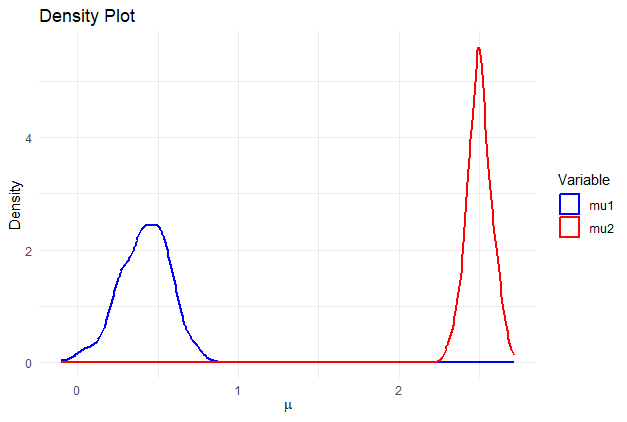
\includegraphics[width=340pt, height=200pt]{Chapters/chapter11/figures/Sim1LSI.png}
	\caption[List of figure caption goes here]{Posterior distributions: Mean parameters, population values $\beta_{01}=0.5$ and $\beta_{02}=1$.}\label{figMean1}
\end{figure}

We perform the same exercise assuming $\beta_{01}=0.5$ and $\beta_{02}=1$. Figure \ref{figMean2} shows the posterior densities, where we observe significant overlap. The posterior means are 0.77 in both cases, with 95\% credible intervals of (0.40, 1.05) and (-0.44, 1.71). The posterior mean of the probability is 0.84. 
 
\begin{figure}[!h]
	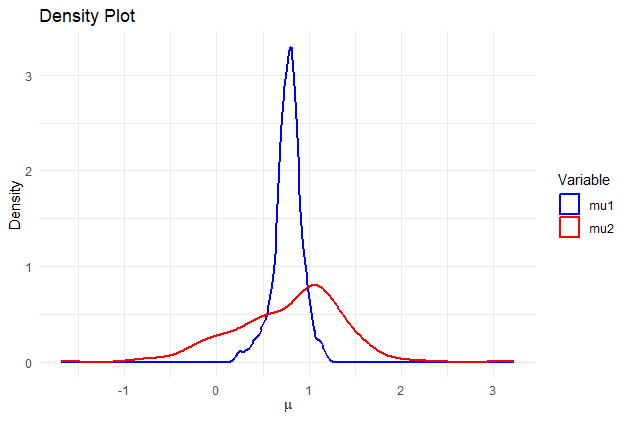
\includegraphics[width=340pt, height=200pt]{Chapters/chapter11/figures/Sim2LSI.png}
	\caption[List of figure caption goes here]{Posterior distributions: Mean parameters, population values $\beta_{01}=0.5$ and $\beta_{02}=1$.}\label{figMean2}
\end{figure}

In the second setting, the posterior draws of the Gibbs sampler can switch between the two means because they are relatively close. This situation contrasts with the first example, where there is a relatively large separation between the means, resulting in a region of the parameter space with zero probability (see the flat region between the two posterior distributions in Figure \ref{figMean1}). The key point is that, given a sufficiently large number of Gibbs sampler iterations, the algorithm should eventually explore the entire parameter space and encounter the label-switching issue. This occurs because both posterior chains should exhibit similar behavior, as they are targeting the same distribution. 

We can implement \textit{random permutation of latent classes} to address this issue. This involves sampling a random permutation of the labels at each iteration of the MCMC algorithm. For example, with three clusters, there are $3! = 6$ possible label permutations. Let the permutations be labeled as $\boldsymbol{p}_k=\left\{p_k(1),p_k(2),\dots,p_k(H)\right\}, k=1,2,\dots,H!$. At the end of each iteration in the MCMC algorithm, we randomly select one of the permutations $\boldsymbol{p}_k$ and replace the cluster probabilities $\lambda_1^{(s)},\dots,\lambda_H^{(s)}$ with $\lambda_{p_k(1)}^{(s)},\dots,\lambda_{p_k(H)}^{(s)}$. We apply the same permutation to $\boldsymbol{\beta}^{(s)}$, $\sigma^{2(s)}$, and $\boldsymbol{\psi}_{i}^{(s)}$, for $i=1,2,\dots,n$. The following algorithm illustrates how to implement this in our simple example.

\begin{tcolorbox}[enhanced,width=4.67in,center upper,
	fontupper=\large\bfseries,drop shadow southwest,sharp corners]
	\textit{R code. Simulation exercise: Random permutation of latent classes}
	\begin{VF}
		\begin{lstlisting}[language=R]
###### Permutations ######
rm(list = ls()); set.seed(010101); library(ggplot2)
# Simulate data from a 2-component mixture model
n <- 500
z <- rbinom(n, 1, 0.75)  # Latent class indicator
y <- ifelse(z == 0, rnorm(n, 0.5, 1), rnorm(n, 2.5, 1))
# Hyperparameters
mu0 <- 0; sig2mu0 <- 10; H <- 2; a0h <- rep(1/H, H)
# MCMC parameters
mcmc <- 2000; burnin <- 500
tot <- mcmc + burnin; thin <- 2
# Gibbs sampling functions
Postmu <- function(yh){
	Nh <- length(yh)
	sig2mu <- (1/sig2mu0 + Nh)^(-1)
	mun <- sig2mu*(mu0/sig2mu0 + sum(yh))
	mu <- rnorm(1, mun, sig2mu^0.5)
	return(mu)
}
PostPsi <- matrix(NA, tot, n); PostMu <- matrix(NA, tot, H)
PostLambda <- rep(NA, tot)
Id1 <- which(y <= 1); Id2 <- which(y > 1)
N1 <- length(Id1); N2 <- length(Id2)
Lambda <- c(N1/n, N2/n); MU <- c(mean(y[Id1]), mean(y[Id2]))
Psi <- rep(NA, n); per1 <- c(1,2); per2 <- c(2,1)
pb <- winProgressBar(title = "progress bar", min = 0, max = tot, width = 300)
for(s in 1:tot){
	for(i in 1:n){
		lambdai <- NULL
		for(h in 1:H){
			lambdaih <- Lambda[h]*dnorm(y[i], MU[h], 1)
			lambdai <- c(lambdai, lambdaih)
		}
		Psi[i] <- sample(1:H, 1, prob = lambdai)
	}
	for(h in 1:H){
		idh <- which(Psi == h)
		MU[h] <- Postmu(yh = y[idh])
	}
	Lambda <- MCMCpack::rdirichlet(1, a0h + table(Psi))
	# Permutations
	labels <- sample(1:2, 1, prob = c(0.5, 0.5))
	if(labels == 2){
		Lambda <- Lambda[per2]
		MU <- MU[per2]
		for(i in 1:n){
			if(Psi[i] == 1){Psi[i] <- 2
			}else{Psi[i] <- 1}
		}
	}
	PostPsi[s, ] <- Psi; PostMu[s,] <- MU
	PostLambda[s] <- Lambda[1]
	setWinProgressBar(pb, s, title=paste( round(s/tot*100, 0),"% done"))
}
close(pb)\end{lstlisting}
	\end{VF}
\end{tcolorbox}

\begin{tcolorbox}[enhanced,width=4.67in,center upper,
	fontupper=\large\bfseries,drop shadow southwest,sharp corners]
	\textit{R code. Simulation exercise: Random permutation of latent classes}
	\begin{VF}
		\begin{lstlisting}[language=R]
keep <- seq(burnin, tot, thin)
PosteriorMUs <- coda::mcmc(PostMu[keep,])
summary(PosteriorMUs)
plot(PosteriorMUs)
dfMU <- data.frame(mu1 = PostMu[keep,1], mu2 = PostMu[keep,2])
# Plot
require(latex2exp)
ggplot(dfMU) +
geom_density(aes(x = mu1, color = "mu1"), linewidth = 1) +  # First density plot
geom_density(aes(x = mu2, color = "mu2"), linewidth = 1) +  # Second density plot
labs(title = "Density Plot", x = TeX("$\\mu$"), y = "Density", color = "Variable") +
theme_minimal() +
scale_color_manual(values = c("mu1" = "blue", "mu2" = "red"))  # Custom colors
PosteriorLAMBDA <- coda::mcmc(PostLambda[keep])
summary(PosteriorLAMBDA)
plot(PosteriorLAMBDA)
		\end{lstlisting}
	\end{VF}
\end{tcolorbox}

Figure \ref{figMeanPerm} shows the posterior distributions from the random permutation of latent classes in the first simulation setting. We observe that both posterior distributions look similar.

\begin{figure}[!h]
	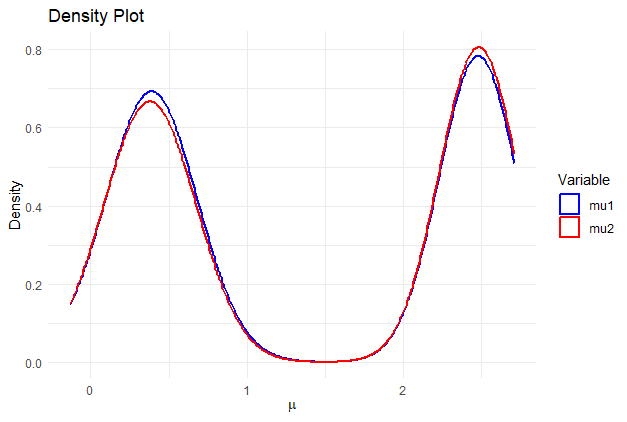
\includegraphics[width=340pt, height=200pt]{Chapters/chapter11/figures/Permutation.png}
	\caption[List of figure caption goes here]{Posterior distributions: Mean parameters, population values $\beta_{01}=0.5$ and $\beta_{02}=2.5$.}\label{figMeanPerm}
\end{figure}
 
In the following setting we simulate a simple regression mixture with two components such that $\psi_{i1}\sim \text{Ber}(0.5)$, consequently, $\psi_{i2}=1-\psi_{i1}$, and assume one regressor, $x_i\sim N(0,1)$, $i=1,2,\dots,1,000$. Then, 
$$p(y_i \mid \boldsymbol{x}_i) = 
0.5 \phi(y_i \mid 2+1.5x_i,1^2)+0.5 \phi(y_i \mid -1+0.5x_i,0.8^2).$$

The following code shows how to perform inference in this model, assuming $N(0,5)$ and $N(0,2)$ priors for the intercepts and slopes, respectively. Additionally, we use a $Cauchy(0,2)$ prior truncated at 0 for the standard deviations, and a $Dirichlet(1,1)$ prior for the probabilities. We use the \textit{brms} package in \textbf{R}, which in turn uses \textit{Stan}, setting number of MCMC iterations 2,000, a burn-in (warm-up) equal to 1,000, and 4 chains. Remember that \textit{Stan} software uses Hamiltonian Monte Carlo.

The following code performs inference in this simulation from scratch using Gibbs sampling. We do not implement the random permutation of latent classes algorithm for facilitating exposition and comparability with the results from the package \textit{brms}. We use non-informative priors, setting $\alpha_{h0}=\delta_{h0}=0.01$, $\boldsymbol{\beta}_{h0}=\boldsymbol{0}_2$, $\boldsymbol{B}_{h0}=\boldsymbol{I}_2$, and $\boldsymbol{\alpha}_0=[1/2 \ 1/2]^{\top}$. The number of MCMC iterations is 5,000, the burn-in is 1,000, and the thinning parameter is 2. In general, the Gibbs sampler appears to yield good posterior results as all 95\% intervals encompass the population parameters. 

\begin{tcolorbox}[enhanced,width=4.67in,center upper,
	fontupper=\large\bfseries,drop shadow southwest,sharp corners]
	\textit{R code. Simulation exercise: Gaussian mixture with 2 components using brms package}
	\begin{VF}
		\begin{lstlisting}[language=R]
####### Simulation exercise: Gaussian mixture: 2 components #############
rm(list = ls())
set.seed(010101)
library(brms)
library(ggplot2)

# Simulate data from a 2-component mixture model
n <- 1000
x <- rnorm(n)
z <- rbinom(n, 1, 0.5)  # Latent class indicator
y <- ifelse(z == 0, rnorm(n, 2 + 1.5*x, 1), rnorm(n, -1 + 0.5*x, 0.8))
data <- data.frame(y, x)

# Plot
ggplot(data, aes(x = y)) +
geom_density(fill = "blue", alpha = 0.3) +  # Density plot with fill color
labs(title = "Density Plot", x = "y", y = "Density") +
theme_minimal()

# Define priors
priors <- c(
set_prior("normal(0, 5)", class = "Intercept", dpar = "mu1"),  # First component intercept
set_prior("normal(0, 5)", class = "Intercept", dpar = "mu2"),  # Second component intercept
set_prior("normal(0, 2)", class = "b", dpar = "mu1"),  # First component slope
set_prior("normal(0, 2)", class = "b", dpar = "mu2"),  # Second component slope
set_prior("cauchy(0, 2)", class = "sigma1", lb = 0),  # First component sigma
set_prior("cauchy(0, 2)", class = "sigma2", lb = 0),  # Second component sigma
set_prior("dirichlet(1, 1)", class = "theta")  # Mixing proportions
)

# Fit a 2-component Gaussian mixture regression model
fit <- brm(
bf(y ~ 1 + x, family = mixture(gaussian, gaussian)),  # Two normal distributions
data = data,
prior = priors,
chains = 4, iter = 2000, warmup = 1000, cores = 4
)
prior_summary(fit) # Summary of priors
summary(fit) # Summary of posterior draws
plot(fit) # Plots of posterior draws
		\end{lstlisting}
	\end{VF}
\end{tcolorbox}

\begin{tcolorbox}[enhanced,width=4.67in,center upper,
	fontupper=\large\bfseries,drop shadow southwest,sharp corners]
	\textit{R code. Simulation exercise: Gaussian mixture with 2 components using Gibbs sampling}
	\begin{VF}
		\begin{lstlisting}[language=R]
########### Perform inference from scratch ###############
rm(list = ls()); set.seed(010101)
library(brms); library(ggplot2)
# Simulate data from a 2-component mixture model
n <- 1000
x <- rnorm(n)
z <- rbinom(n, 1, 0.5)  # Latent class indicator
y <- ifelse(z == 0, rnorm(n, 2 + 1.5*x, 1), rnorm(n, -1 + 0.5*x, 0.8))
# Hyperparameters
d0 <- 0.001; a0 <- 0.001
b0 <- rep(0, 2); B0 <- diag(2); B0i <- solve(B0)
a01 <- 1/2; a02 <- 1/2
# MCMC parameters
mcmc <- 5000; burnin <- 1000
tot <- mcmc + burnin; thin <- 2
# Gibbs sampling functions
PostSig2 <- function(Betah, Xh, yh){
	Nh <- length(yh); an <- a0 + Nh
	dn <- d0 + t(yh - Xh%*%Betah)%*%(yh - Xh%*%Betah)
	sig2 <- invgamma::rinvgamma(1, shape = an/2, rate = dn/2)
	return(sig2)
}
PostBeta <- function(sig2h, Xh, yh){
	Bn <- solve(B0i + sig2h^(-1)*t(Xh)%*%Xh)
	bn <- Bn%*%(B0i%*%b0 + sig2h^(-1)*t(Xh)%*%yh)
	Beta <- MASS::mvrnorm(1, bn, Bn)
	return(Beta)
}
PostBetas1 <- matrix(0, mcmc+burnin, 2)
PostBetas2 <- matrix(0, mcmc+burnin, 2)
PostSigma21 <- rep(0, mcmc+burnin)
PostSigma22 <- rep(0, mcmc+burnin)
PostPsi <- matrix(0, mcmc+burnin, n)
PostLambda <- rep(0, mcmc+burnin)
Id1 <- which(y<1) # 1 is from inspection of the density plot of y 
N1 <- length(Id1); Lambda1 <- N1/n
Id2 <- which(y>=1)
N2 <- length(Id2); Lambda2 <- N2/n
Reg1 <- lm(y ~ x, subset = Id1)
SumReg1 <- summary(Reg1); Beta1 <- Reg1$coefficients
sig21 <- SumReg1$sigma^2 
Reg2 <- lm(y ~ x, subset = Id2); SumReg2 <- summary(Reg2)
Beta2 <- Reg2$coefficients
sig22 <- SumReg2$sigma^2
X <- cbind(1, x); Psi <- rep(NA, n)
\end{lstlisting}
	\end{VF}
\end{tcolorbox}
 
\begin{tcolorbox}[enhanced,width=4.67in,center upper,
	fontupper=\large\bfseries,drop shadow southwest,sharp corners]
	\textit{R code. Simulation exercise: Gaussian mixture with 2 components using Gibbs sampling}
	\begin{VF}
		\begin{lstlisting}[language=R]
pb <- winProgressBar(title = "progress bar", min = 0, max = tot, width = 300)
for(s in 1:tot){
	for(i in 1:n){
		lambdai1 <- Lambda1*dnorm(y[i], X[i,]%*%Beta1, sig21^0.5)
		lambdai2 <- Lambda2*dnorm(y[i], X[i,]%*%Beta2, sig22^0.5)
		Psi[i] <- sample(c(1,2), 1, prob = c(lambdai1, lambdai2))
	}
	PostPsi[s, ] <- Psi
	Id1 <- which(Psi == 1); Id2 <- which(Psi == 2)
	N1 <- length(Id1); N2 <- length(Id2)
	sig21 <- PostSig2(Betah = Beta1, Xh = X[Id1, ], yh = y[Id1])
	sig22 <- PostSig2(Betah = Beta2, Xh = X[Id2, ], yh = y[Id2])
	PostSigma21[s] <- sig21; PostSigma22[s] <- sig22
	Beta1 <- PostBeta(sig2h = sig21, Xh = X[Id1, ], yh = y[Id1])
	Beta2 <- PostBeta(sig2h = sig22, Xh = X[Id2, ], yh = y[Id2])
	PostBetas1[s,] <- Beta1; PostBetas2[s,] <- Beta2
	Lambda <- sort(MCMCpack::rdirichlet(1, c(a01 + N1, a02 + N2)), decreasing = TRUE)
	Lambda1 <- Lambda[1]; Lambda2 <- Lambda[2]
	PostLambda[s] <- Lambda1 
  setWinProgressBar(pb, s, title=paste( round(s/tot*100, 0),"% done"))
}
close(pb)
keep <- seq((burnin+1), tot, thin)
PosteriorBetas1 <- coda::mcmc(PostBetas1[keep,])
summary(PosteriorBetas1)
plot(PosteriorBetas1)
PosteriorBetas2 <- coda::mcmc(PostBetas2[keep,])
summary(PosteriorBetas2)
plot(PosteriorBetas2)
PosteriorSigma21 <- coda::mcmc(PostSigma21[keep])
summary(PosteriorSigma21)
plot(PosteriorSigma21)
PosteriorSigma22 <- coda::mcmc(PostSigma22[keep])
summary(PosteriorSigma22)
plot(PosteriorSigma22)
\end{lstlisting}
	\end{VF}
\end{tcolorbox}

Let's perform another simulation exercise in which we conduct a semi-parametric analysis where the stochastic error follows a Student's t-distribution with 3 degrees of freedom. Specifically,  
\begin{align*}
	y_i &= 1 - 0.5x_{i1} + 1.5x_{i2} + \mu_i, \ i=1,2,\dots,500.
\end{align*}
The variables $x_{i1}$ and $x_{i2}$ are standard normally distributed. Let's set $H=5$, and use non-informative priors setting $\alpha_{h0}=\delta_{h0}=0.01$, $\boldsymbol{\beta}_0=\boldsymbol{0}_2$, $\boldsymbol{B}_0=\boldsymbol{I}_2$, $\mu_{h0}=0$, $\sigma^2_{\mu 0}=10$ and $\boldsymbol{\alpha}_0=[1/H \ \dots \ 1/H]^{\top}$. Use 6,000 MCMC iterations, burn-in equal to 4,000, and thinning parameter equal to 2. In this exercise, there is no need to address the label-switching issue, as we are not specifically interested in the individual components of the posterior distributions of the clusters. Exercise 1 asks how to get the posterior density of the stochastic errors in this semi-parametric specifications. 

We can see from the posterior estimates that three components disappear after the burn-in iterations. The 95\% credible intervals encompass the population values of the slope parameters. The 95\% credible intervals for the probabilities are (0.70, 0.89) and (0.11, 0.30), and the 95\% credible interval for the weighted average of the intercepts encompasses the population parameter.

\begin{tcolorbox}[enhanced,width=4.67in,center upper,
	fontupper=\large\bfseries,drop shadow southwest,sharp corners]
	\textit{R code. Simulation exercise: Semi-parametric model using Gibbs sampling}
	\begin{VF}
		\begin{lstlisting}[language=R]
rm(list = ls()); set.seed(010101)
library(ggplot2)
# Simulate data from a 2-component mixture model
n <- 500
x1 <- rnorm(n); x2 <- rnorm(n)
X <- cbind(x1,x2); B <- c(-0.5, 1.5)
u <- rt(n, 3); y <- 1 + X%*%B + u
Reg <- lm(y ~ X)
Res <- Reg$residuals
data <- data.frame(Res)
# Plot
ggplot(data, aes(x = Res)) +
geom_density(fill = "blue", alpha = 0.3) +  # Density plot with fill color
labs(title = "Density Plot", x = "Residuals", y = "Density") +
theme_minimal()
# Hyperparameters
d0 <- 0.001; a0 <- 0.001; b0 <- rep(0, 2)
B0 <- diag(2); B0i <- solve(B0)
mu0 <- 0; sig2mu0 <- 10; H <- 5; a0h <- rep(1/H, H)
# MCMC parameters
mcmc <- 2000; burnin <- 4000
tot <- mcmc + burnin; thin <- 2
# Gibbs sampling functions
PostSig2 <- function(Beta, muh, Xh, yh){
	Nh <- length(yh); an <- a0 + Nh
	dn <- d0 + t(yh - muh - Xh%*%Beta)%*%(yh - muh - Xh%*%Beta)
	sig2 <- invgamma::rinvgamma(1, shape = an/2, rate = dn/2)
	return(sig2)
}
PostBeta <- function(sig2, mu, X, y, Psi){
	XtX <- matrix(0, 2, 2); Xty <- matrix(0, 2, 1)
	Hs <- length(mu)
	for(h in 1:Hs){
		idh <- which(Psi == h)
		if(length(idh) == 1){
			Xh <- matrix(X[idh,], 1, 2)
			XtXh <- sig2[h]^(-1)*t(Xh)%*%Xh
			yh <- y[idh]
			Xtyh <- sig2[h]^(-1)*t(Xh)%*%(yh - mu[h])
		}else{
			Xh <- X[idh,]
			XtXh <- sig2[h]^(-1)*t(Xh)%*%Xh
			yh <- y[idh]
			Xtyh <- sig2[h]^(-1)*t(Xh)%*%(yh - mu[h])
		}
		XtX <- XtX + XtXh; Xty <- Xty + Xtyh
	}
	Bn <- solve(B0i + XtX); bn <- Bn%*%(B0i%*%b0 + Xty)
	Beta <- MASS::mvrnorm(1, bn, Bn)
	return(Beta)
}
\end{lstlisting}
	\end{VF}
\end{tcolorbox}

\begin{tcolorbox}[enhanced,width=4.67in,center upper,
	fontupper=\large\bfseries,drop shadow southwest,sharp corners]
	\textit{R code. Simulation exercise: Semi-parametric model using Gibbs sampling}
	\begin{VF}
		\begin{lstlisting}[language=R]
Postmu <- function(sig2h, Beta, Xh, yh){
	Nh <- length(yh)
	sig2mu <- (1/sig2mu0 + Nh/sig2h)^(-1)
	mun <- sig2mu*(mu0/sig2mu0 + sum((yh - Xh%*%Beta))/sig2h)
	mu <- rnorm(1, mun, sig2mu^0.5)
	return(mu)
}
PostBetas <- matrix(0, mcmc+burnin, 2)
PostPsi <- matrix(0, mcmc+burnin, n)
PostSigma2 <- list(); PostMu <- list()
PostLambda <- list()
Resq <- quantile(Res, c(0.2, 0.4, 0.6, 0.8))
Id1 <- which(Res <= Resq[1])
Id2 <- which(Res > Resq[1] & Res <= Resq[2])
Id3 <- which(Res > Resq[2] & Res <= Resq[3])
Id4 <- which(Res > Resq[3] & Res <= Resq[4])
Id5 <- which(Res > Resq[4])
Nh <- rep(n/H, H); Lambda <- rep(1/H, H)
MU <- c(mean(Res[Id1]), mean(Res[Id2]), mean(Res[Id3]), mean(Res[Id4]), mean(Res[Id5]))
Sig2 <- c(var(Res[Id1]), var(Res[Id2]), var(Res[Id3]), var(Res[Id4]), var(Res[Id5]))
Beta <- Reg$coefficients[2:3]
Psi <- rep(NA, n); Hs <- length(MU)
pb <- winProgressBar(title = "progress bar", min = 0, max = tot, width = 300)
for(s in 1:tot){
	for(i in 1:n){
		lambdai <- NULL
		for(h in 1:Hs){
			lambdaih <- Lambda[h]*dnorm(y[i] - X[i,]%*%Beta, MU[h], Sig2[h]^0.5)
			lambdai <- c(lambdai, lambdaih)
		}
		Psi[i] <- sample(1:Hs, 1, prob = lambdai)
	}
	PostPsi[s, ] <- Psi
	Hs <- length(table(Psi))
	for(h in 1:Hs){
		idh <- which(Psi == h)
		Sig2[h] <- PostSig2(Beta = Beta, muh = MU[h], Xh = X[idh,], yh = y[idh])
		MU[h] <- Postmu(sig2h = Sig2[h], Beta = Beta, Xh = X[idh,], yh = y[idh])
	}
	PostSigma2[[s]] <- Sig2
	PostMu[[s]] <- MU 
	Beta <- PostBeta(sig2 = Sig2, mu = MU, X = X, y = y, Psi = Psi)
	PostBetas[s,] <- Beta
	Lambda <- sort(MCMCpack::rdirichlet(1, a0h[1:Hs] + table(Psi)), decreasing = TRUE)
	PostLambda[[s]] <- Lambda
	setWinProgressBar(pb, s, title=paste( round(s/tot*100, 0),"% done"))
}
close(pb)
\end{lstlisting}
	\end{VF}
\end{tcolorbox}

\begin{tcolorbox}[enhanced,width=4.67in,center upper,
	fontupper=\large\bfseries,drop shadow southwest,sharp corners]
	\textit{R code. Simulation exercise: Semi-parametric model using Gibbs sampling}
	\begin{VF}
		\begin{lstlisting}[language=R]
keep <- seq(burnin, tot, thin)
PosteriorBetas <- coda::mcmc(PostBetas[keep,])
summary(PosteriorBetas)
plot(PosteriorBetas)
PosteriorPsi <- PostPsi[keep,]
Clusters <- sapply(1:length(keep), function(i){length(table(PosteriorPsi[i,]))})
NClus <- 2
PosteriorSIGMA <- matrix(NA, length(keep), NClus)
PosteriorMU <- matrix(NA, length(keep), NClus)
PosteriorLAMBDA <- matrix(NA, length(keep), NClus)
l <- 1
for (s in keep){
	PosteriorSIGMA[l,] <- PostSigma2[[s]][1:NClus]
	PosteriorMU[l,] <- PostMu[[s]][1:NClus]
	PosteriorLAMBDA[l,] <- PostLambda[[s]][1:NClus]
	l <- l + 1
}

summary(coda::mcmc(PosteriorSIGMA))
summary(coda::mcmc(PosteriorMU))
summary(coda::mcmc(PosteriorLAMBDA))
\end{lstlisting}
	\end{VF}
\end{tcolorbox}


\subsection{Direchlet processes}\label{sec11_12}

A Dirichlet process (DP) is a probability distribution over probability distributions, and a generalization of the Dirichlet distribution. It was introduced by \cite{Ferguson1973}, and it is commonly used as a prior for unknown distributions, making it particularly useful in non-parametric settings. Unlike finite Gaussian mixture models, a Dirichlet process does not require pre-specifying the number of components, allowing for greater flexibility in modeling complex data structures. In this sense, DPs can be viewed as the limiting case of finite mixtures when the number of components approaches infinity. 

A Dirichlet process $G\sim DP(\alpha G_0)$ is defined by a precision parameter $\alpha>0$, and a base probability measure $G_0$ on a probability space $\Omega$.\footnote{Measurability ensures that we can compute probabilities and expectations properly. If a set is not measurable, we cannot define its probability meaningfully.} The DP assigns probability $G(B)$ to any (measurable) set $B$ in $\Omega$ such that for any finite (measurable) partition $\left\{B_1, B_2, \dots, B_k\right\}$ of $\Omega$,  

\[
G(B_1), G(B_2), \dots, G(B_k) \sim \text{Dirichlet}(\alpha G_0(B_1), \alpha G_0(B_2), \dots, \alpha G_0(B_k)).
\]

In particular, $\mathbb{E}\left[G(B)\right]=G_0(B)$ and $\mathbb{V}ar\left[G(B)\right]=G_0(B)\left[1-G_0(B)\right]/(1+\alpha)$ \cite[p.~8]{Muller2015}. Observe that as $\alpha  \rightarrow \infty$, $G$ concentrates at $G_0$, which is why $\alpha$ is called the precision parameter.

A key property of the DP is its discrete nature, which allows it to be expressed as  
\[
G(\cdot)=\sum_{h=1}^{\infty}\lambda_h\delta_{\boldsymbol{\theta}_h}(\cdot),
\]
where $\lambda_h$ is the probability mass at $\boldsymbol{\theta}_h$, and $\delta_{\boldsymbol{\theta}_h}(\cdot)$ denotes the Dirac measure that assigns mass one to the atom $\boldsymbol{\theta}_h$.\footnote{An atom is a set that has positive probability but cannot be further decomposed into smaller sets with strictly smaller probability.} Given this property, a particularly useful construction of the DP is the \textit{stick-breaking} representation \cite{Sethuraman1994}, which is given by  
\begin{align*}
	G(\cdot)&=\sum_{h=1}^{\infty}\lambda_h\delta_{\boldsymbol{\theta}_h}(\cdot),\\
	\lambda_h&=V_h\prod_{m<h}(1-V_m), \quad V_h\sim \text{Beta}(1,\alpha),\\
	\boldsymbol{\theta}_h&\stackrel{iid}{\sim} G_0.
\end{align*}  

The intuition behind this representation is straightforward. We begin with a stick of length 1 and break off a random proportion $V_1$ drawn from a $\text{Beta}(1,\alpha)$ distribution. This assigns a probability mass of $\lambda_1=V_1$ to $\boldsymbol{\theta}_1$, which is sampled from $G_0$. Next, from the remaining stick of length $(1-V_1)$, we break off a fraction proportional to $V_2 \sim \text{Beta}(1,\alpha)$, assigning a probability mass of $\lambda_2=V_2(1-V_1)$ to a new draw $\boldsymbol{\theta}_2$ from $G_0$. This process continues indefinitely. 

Since $\mathbb{E}(V_h) = \frac{1}{1+\alpha}$, as $\alpha \rightarrow \infty$, we have $\mathbb{E}(V_h) \rightarrow 0$. Consequently, the DP places mass on a large number of atoms, leading to convergence to the base distribution $G_0$.  

An important limitation of the DP is that its realizations are discrete distributions, which poses challenges when working with continuous distributions. One way to overcome this limitation is to use the DP as a mixing distribution for simple parametric distributions, such as the normal distribution \cite{Escobar1995}. This leads to Dirichlet process mixtures (DPM), which are defined as  
\begin{align*}
	f_G(y) &= \int f_{\boldsymbol{\theta}}(y) dG(\boldsymbol{\theta}).
\end{align*}

Observe that the mixing measure $G$ is discrete when a DP is the prior, with mass concentrated at an infinite number of atoms $\boldsymbol{\theta}_h$. Consequently, if $f_{\boldsymbol{\theta}}(y)$ follows a Gaussian distribution, the resulting mixture resembles a finite Gaussian mixture. However, unlike finite mixtures, the DP-based approach eliminates the need to pre-specify the number of components, as it provides an automatic mechanism for determining them.

Thus, if we assume $y\sim N(\boldsymbol{x}_i^{\top}\boldsymbol{\beta},\sigma^2)$, then the DPM is 
\[
p(y_i \mid \{\lambda_h, \boldsymbol{\beta}_h, \sigma_h^2\}_{h=1}^{\infty}, \boldsymbol{x}_i) = 
\sum_{h=1}^{\infty} \lambda_h \phi(y_i \mid \boldsymbol{x}_i^{\top}\boldsymbol{\beta}_h, \sigma_h^2),
\]
where $\lambda_h$ are drawn from the stick-breaking representation of the DP, and $\boldsymbol{\theta}_h=[\boldsymbol{\beta}_h^{\top} \ \sigma^2_h]^{\top}$.

This mixture model can be expressed in a hierarchical structure:
\begin{align*}
	y_i\mid \boldsymbol{\theta}_i & \stackrel{ind}{\sim}f_{\boldsymbol{\theta}_i}\\
	\boldsymbol{\theta}_i \mid G & \stackrel{iid}{\sim} G\\
	G \mid \alpha,G_0 & \sim DP(\alpha G_0).
\end{align*}

Note that the hierarchical representation induces specific unit parameters, leading to a probabilistic clustering model \cite{Antoniak1974}, similar to a finite Gaussian mixture. However, the DPM is not consistent in estimating the number of clusters, it tends to overestimate the number of clusters (see simulation exercise below); although there is posterior asymptotic concentration in the other model components \cite{Miller2014}.

The hierarchical representation implies that there are latent assignment variables \( s_i = h \), such that when \( \boldsymbol{\theta}_i \) is equal to the \( h \)-th unique \( \boldsymbol{\theta}_h^* \) — that is, \( \boldsymbol{\theta}_i = \boldsymbol{\theta}_h^* \)— then \( s_i = h \). Then,
\begin{align*}
	s_i&\sim \sum_{h=0}^{\infty}\lambda_h\delta_h,\\
	y_i\mid s_i, \boldsymbol{\theta}_{s_i}&\sim N(\boldsymbol{x}_i^{\top}\boldsymbol{\beta}_{s_i},\sigma^2_{s_i}),
\end{align*} 
where $\lambda_h=P(\boldsymbol{\theta}_{i}=\boldsymbol{\theta}_{h}^*)$.

This latent assignment structure, the \textit{Pólya urn} representation of the DP \cite{Blackwell1973}, which is obtained when \( G \) is marginalized out to avoid infinite atoms, and the use of conjugate priors allow for convenient computational inference in DPM.

Specifically, we assume $\boldsymbol{\beta}_i\mid \sigma^2_i\sim N(\boldsymbol{\beta}_0, \sigma^2_i\boldsymbol{B}_0)$ and $\sigma_i^2\sim IG(\alpha_0/2,\delta_0/2)$. In addition, we can add a layer in the hierarchical representation, $\alpha\sim G(a,b)$ such that introducing the latent variable $\xi|\alpha,N\sim Be(\alpha+1,N)$, allows to easily sample the posterior draws of  $\alpha|\xi,H,\pi_{\xi}\sim\pi_{\xi}{G}(a+H,b-log(\xi))+(1-\pi_{\xi}){G}(a+H-1,b-log(\xi))$, where $\frac{\pi_{\xi}}{1-\pi_{\xi}}=\frac{a+H-1}{N(b-log(\xi))}$, $H$ is the number of atoms (mixture components) \cite{Escobar1995}. 

The conditional posterior distribution of $\boldsymbol\theta_i$ is
\begin{align*}
	\boldsymbol\theta_i|\left\{\boldsymbol\theta_{i'},\boldsymbol s_{i'}:i'\neq i\right\}, y_i, \alpha & \sim \sum_{i'\neq i}\frac{N_h^{(i)}}{\alpha+N-1}f_N(y_i|\boldsymbol{x}_i^{\top}\boldsymbol{\beta}_h,\sigma_h^2)\\
	& +\frac{\alpha}{\alpha+N-1}\int_{\mathcal{R}^K}\int_{0}^{\infty}f_N(y_i|\boldsymbol{x}_i^{\top}\boldsymbol{\beta},\sigma^2)f_N\left(\boldsymbol\beta\Big|\boldsymbol\beta_0,\sigma^2\boldsymbol B_0\right)f_{IG}(\sigma^2|\alpha_0,\delta_0)d\sigma^2 d\boldsymbol\beta,
\end{align*}
where $N_h^{(i)}$ is the number of observations such that $s_{i'}=h$, $i'\neq i$.

Observe that the probability of belonging to a particular cluster has a reinforcement property, as it increases with the cluster size; therefore, a DPM exhibits a self-reinforcing property, the more often a given value has been sampled in the past, the more likely it is to be sampled again.

Observe that the integral in the previous equation has exactly the same form as in the marginal likelihood presented in Section \ref{sec43}. Thus,
\begin{align*}
	p(y_i)&=\int_{\mathcal{R}^K}\int_{0}^{\infty}f_N(y_i|\boldsymbol{x}_i^{\top}\boldsymbol{\beta},\sigma^2)f_N\left(\boldsymbol\beta\Big|\boldsymbol\beta_0,\sigma^2\boldsymbol B_0\right)f_{IG}(\sigma^2|\alpha_0,\delta_0)d\sigma^2 d\boldsymbol\beta\\
	&=\frac{1}{\pi^{1/2}}\frac{\delta_0^{\alpha_0/2}}{\delta_n^{\alpha_n/2}}\frac{|{\boldsymbol{B}}_n|^{1/2}}{|{\boldsymbol{B}}_0|^{1/2}}\frac{\Gamma(\alpha_n/2)}{\Gamma(\alpha_0/2)}, 
\end{align*}
where $\alpha_n=1+\alpha_0$, $\delta_n=\delta_0 + y^{\top}y + \boldsymbol{\beta}_0^{\top}{\boldsymbol{B}}_0^{-1}\boldsymbol{\beta}_0 - \boldsymbol{\beta}_n^{\top}{\boldsymbol{B}}_n^{-1}\boldsymbol{\beta}_n$,  $\boldsymbol{B}_n = (\boldsymbol{B}_0^{-1} + \boldsymbol{x}\boldsymbol{x}^{\top})^{-1}$ and $\boldsymbol{\beta}_n = \boldsymbol{B}_n(\boldsymbol{B}_0^{-1}\boldsymbol{\beta}_0 + \boldsymbol{x}y)$.

Therefore, we sample $s_i$ as follows,
\begin{equation*}
	s_i|\left\{\boldsymbol\beta_{i'},\sigma_{i'}^2,\boldsymbol s_{i'}:i'\neq i\right\}, y_i, \alpha\sim\begin{Bmatrix}P(s_i=0|\cdot)=q_0^*\\
		P(s_i=h|\cdot)=q_h^*, h=1,2,\dots,H^{(i)}\end{Bmatrix},
\end{equation*}

where $H^{(i)}$ is the number of clusters excluding $i$, which may have its own cluster (singleton cluster), $q^*_c=\frac{q_c}{q_0+\sum_h q_h}$, $q_c=\left\{q_0,q_h\right\}$, $q_h=\frac{N_h^{(i)}}{\alpha+N-1}f_N(y_i|\boldsymbol{x}_i^{\top}\boldsymbol\beta_h,\sigma_h^2)$ and $q_0=\frac{\alpha}{\alpha+N-1}p(y_i)$.

If $s_i=0$ is sampled, then $s_i=H+1$, and a new $\sigma_h^2$ is sampled from $IG\left(\alpha_n/2,\delta_n/2\right)$, a new $\boldsymbol\beta_h$ is sample from $N(\boldsymbol\beta_n,\sigma_h^2\boldsymbol B_n)$.

Discarding $\boldsymbol\theta_h$'s from last step, we use $\boldsymbol s$ and total number of components to sample $\sigma_h^2$ from 

\begin{equation*}
	IG\left(\frac{\alpha_0+N_m}{2},\frac{\delta_0+\boldsymbol y_h^{\top}\boldsymbol y_h+\boldsymbol{\beta}_0^{\top}{\boldsymbol{B}}_0^{-1}\boldsymbol{\beta}_0-\boldsymbol{\beta}_{hn}^{\top}{\boldsymbol{B}}_{hn}^{-1}\boldsymbol{\beta}_{hn}}{2}\right),
\end{equation*}

where $\boldsymbol{B}_{hn}=(\boldsymbol{B}_0^{-1}+\boldsymbol{X}_h^{\top}\boldsymbol{X}_h)^{-1}$ and $\boldsymbol{\beta}_{hn}=\boldsymbol{B}_{hn}(\boldsymbol{B}_0^{-1}\boldsymbol{\beta}_0+\boldsymbol{X}_h^{\top}\boldsymbol{y}_h)$, $\boldsymbol{X}_h$ and $\boldsymbol{y}_h$ have the $\boldsymbol{x}_i$ and $y_i$ of individuals in component $h$. We sample $\boldsymbol\beta_h$ from
\begin{equation*}
	N\left({\boldsymbol\beta}_{hn},\sigma_h^2\boldsymbol B_{hn}\right),
\end{equation*}
$h=1,2,\dots,H$.

In Exercise 3 we ask to get the posterior sampler in the semi-parameteric setting, that is,
\begin{align*}
	y_i&=\boldsymbol{x}_i^{\top}\boldsymbol{\beta}+e_i\\
	e_i\mid \mu_i,\sigma_i^2 &\stackrel{iid}{\sim} N(\mu_i,\sigma_i^2).
\end{align*}
We should not include the intercept in $\boldsymbol{\beta}$ to get flexibility in the distribution of the stochastic errors. 

To sum up, a Dirichlet process mixture is a flexible way to model non-parametrically a distribution using an infinite weighted sum of discrete distributions, where each individual weight increases with the number of observations that belongs to it.

\textbf{Example: Simulation exercises}

Let's simulate again the simple regression mixture with two components such that $\psi_{i1}\sim \text{Ber}(0.5)$, consequently, $\psi_{i2}=1-\psi_{i1}$, and assume one regressor, $x_i\sim N(0,1)$, $i=1,2,\dots,1,000$. Then, 
$$p(y_i \mid \boldsymbol{x}_i) = 
0.5 \phi(y_i \mid 2+1.5x_i,1^2)+0.5 \phi(y_i \mid -1+0.5x_i,0.8^2).$$

We use non-informative priors again, setting $\alpha_{0}=\delta_{0}=0.01$, $\boldsymbol{\beta}_{0}=\boldsymbol{0}_2$, $\boldsymbol{B}_{0}=\boldsymbol{I}_2$, and $a=b=0.1$. The number of MCMC iterations is 5,000, the burn-in is 1,000, and the thinning parameter is 2. However, we do not have to fix in advance the number of clusters using the DPM.

The following code demonstrates how to perform inference using the stated Gibbs sampler for the DPM in the \textbf{R} package.

We see from the results that the DPM overestimates the number of clusters. After the burn-in period, there are typically three clusters. Additionally, the posterior plots illustrate the label-switching problem. Eventually, the posterior chains of clusters reach different posterior modes, causing a high variability of the posterior draws. In Exercise 5, we ask to fix this issue using \textit{random permutation of latent classes}.

\begin{tcolorbox}[enhanced,width=4.67in,center upper,
	fontupper=\large\bfseries,drop shadow southwest,sharp corners]
	\textit{R code. Simulation exercise: Dirichlet process mixture using Gibbs sampling}
	\begin{VF}
		\begin{lstlisting}[language=R]
rm(list = ls())
set.seed(010101)
# Simulate data from a 2-component mixture model
N <- 1000; x <- rnorm(N); z <- rbinom(N, 1, 0.5)
y <- ifelse(z == 0, rnorm(N, 2 + 1.5*x, 1), rnorm(N, -1 + 0.5*x, 0.8))
X <- cbind(1, x)
k <- 2
data <- data.frame(y, x); Reg <- lm(y ~ x)
SumReg <- summary(Reg)
# Hyperparameters
a0 <- 0.001; d0 <- 0.001
b0 <- rep(0, k); B0 <- diag(k)
B0i <- solve(B0)
a <- 0.1; b <- 0.1
# MCMC parameters
mcmc <- 5000; burnin <- 1000
tot <- mcmc + burnin; thin <- 2
# Gibbs sampling functions
PostSig2 <- function(Xh, yh){
	Nh <- length(yh)
	yh <- matrix(yh, Nh, 1)
	if(Nh == 1){
		Xh <- matrix(Xh, k, 1)
		Bn <- solve(Xh%*%t(Xh) + B0i)
		bn <- Bn%*%(B0i%*%b0 + Xh%*%yh)
	}else{
		Xh <- matrix(Xh, Nh, k)
		Bn <- solve(t(Xh)%*%Xh + B0i)
		bn <- Bn%*%(B0i%*%b0 + t(Xh)%*%yh)
	}
	Bni <- solve(Bn)
	an <- a0 + Nh
	dn <- d0 + t(yh)%*%yh + t(b0)%*%B0i%*%b0 - t(bn)%*%Bni%*%bn 
	sig2 <- invgamma::rinvgamma(1, shape = an/2, rate = dn/2)
	return(sig2)
}
PostBeta <- function(sig2h, Xh, yh){
	Nh <- length(yh)
	yh <- matrix(yh, Nh, 1)
	if(Nh == 1){
		Xh <- matrix(Xh, k, 1)
		Bn <- solve(Xh%*%t(Xh) + B0i)
		bn <- Bn%*%(B0i%*%b0 + Xh%*%yh)
	}else{
		Xh <- matrix(Xh, Nh, k)
		Bn <- solve(t(Xh)%*%Xh + B0i)
		bn <- Bn%*%(B0i%*%b0 + t(Xh)%*%yh)
	}
	Beta <- MASS::mvrnorm(1, bn, sig2h*Bn)
	return(Beta)
}
\end{lstlisting}
	\end{VF}
\end{tcolorbox}

\begin{tcolorbox}[enhanced,width=4.67in,center upper,
	fontupper=\large\bfseries,drop shadow southwest,sharp corners]
	\textit{R code. Simulation exercise: Dirichlet process mixture using Gibbs sampling}
	\begin{VF}
		\begin{lstlisting}[language=R]
PostAlpha <- function(s, alpha){
	H <- length(unique(s))
	psi <- rbeta(1, alpha + 1, N)
	pi.ratio <- (a + H - 1) / (N * (b - log(psi)))
	pi <- pi.ratio / (1 + pi.ratio)
	components <- sample(1:2, prob = c(pi, (1 - pi)), size = 1)
	cs <- c(a + H, a + H - 1)
	ds <- b - log(psi)
	alpha <- rgamma(1, cs[components], ds)
	return(alpha)
}
LogMarLikLM <- function(xh, yh){
	xh <- matrix(xh, k, 1)
	Bn <- solve(xh%*%t(xh) + B0i)
	Bni <- solve(Bn)
	bn <- Bn%*%(B0i%*%b0 + xh%*%yh)
	an <- a0 + 1
	dn <- d0 + yh^2 + t(b0)%*%B0i%*%b0 - t(bn)%*%Bni%*%bn 
	# Log marginal likelihood
	logpy <- (1/2)*log(1/pi)+(a0/2)*log(d0)-(an/2)*log(dn) + 0.5*log(det(Bn)/det(B0)) + lgamma(an/2)-lgamma(a0/2)
	return(logpy)
}
PostS <- function(BETA, SIGMA, Alpha, s, i){
	Nl <- table(s[-i]); H <- length(Nl)
	qh <- sapply(1:H, function(h){(Nl[h]/(N+Alpha-1))*dnorm(y[i], mean = t(X[i,])%*%BETA[,h], sd = SIGMA[h])})
	q0 <- (Alpha/(N+Alpha-1))*exp(LogMarLikLM(xh = X[i,], yh = y[i]))
	qh <- c(q0, qh)
	Clust <- as.numeric(names(Nl))
	si <- sample(c(0, Clust), 1, prob = qh)
		if(si == 0){
			si <- Clust[H] + 1
			Sig2New <- PostSig2(Xh = X[i,], yh = y[i])
			SIGMA <- c(SIGMA, Sig2New^0.5)
			BetaNew <- PostBeta(sig2h = Sig2New, Xh = X[i,], yh = y[i])
			BETA <- cbind(BETA, BetaNew)
		}else{si == si
		}
		return(list(si = si, BETA = BETA, SIGMA = SIGMA))
	}
PostBetas <- list(); PostSigma <- list()
Posts <- matrix(0, tot, N); PostAlphas <- rep(0, tot)
S <- sample(1:3, N, replace = T, prob = c(0.5, 0.3, 0.2))
BETA <- cbind(Reg$coefficients, Reg$coefficients, Reg$coefficients)
SIGMA <- rep(SumReg$sigma, 3)
Alpha <- rgamma(1, a, b)
\end{lstlisting}
	\end{VF}
\end{tcolorbox}

\begin{tcolorbox}[enhanced,width=4.67in,center upper,
	fontupper=\large\bfseries,drop shadow southwest,sharp corners]
	\textit{R code. Simulation exercise: Dirichlet process mixture using Gibbs sampling}
	\begin{VF}
		\begin{lstlisting}[language=R]
pb <- winProgressBar(title = "progress bar", min = 0, max = tot, width = 300)
for(s in 1:tot){
	for(i in 1:N){
		Rests <- PostS(BETA = BETA, SIGMA = SIGMA, Alpha = Alpha, s = S, i = i)
		S[i] <- Rests$si
		BETA <- Rests$BETA; SIGMA <- Rests$SIGMA
	}
  	sFreq <- table(S)
	lt <- 1
	for(li in as.numeric(names(sFreq))){
		Index <- which(S == li)
		if(li == lt){S[Index] <- li
		} else {S[Index] <- lt
		}
		lt <- lt + 1
	}
	Alpha <- PostAlpha(s = S, alpha = Alpha)
	Nl <- table(S); H <- length(Nl)
	SIGMA <- rep(NA, H)
	BETA <- matrix(NA, k, H)
	l <- 1
	for(h in unique(S)){
		Idh <- which(S == h)
		SIGMA[l] <- (PostSig2(Xh = X[Idh, ], yh = y[Idh]))^0.5
		BETA[,l] <- PostBeta(sig2h = SIGMA[l]^2, Xh = X[Idh, ], yh = y[Idh])
		l <- l + 1
	}
	PostBetas[[s]] <- BETA
	PostSigma[[s]] <- SIGMA
	Posts[s, ] <- S
	PostAlphas[s] <- Alpha
	setWinProgressBar(pb, s, title=paste( round(s/tot*100, 0),"% done"))
}
close(pb)
keep <- seq((burnin+1), tot, thin)
PosteriorS<- Posts[keep,]
Clusters <- sapply(1:length(keep), function(i){length(table(PosteriorS[i,]))})
table(Clusters)
PosteriorBeta1 <- matrix(NA, length(keep), k); j <- 1
for(s in keep){
	PosteriorBeta1[j,] <- PostBetas[[s]][,1]; j <- j + 1
}
print(summary(coda::mcmc(PosteriorBeta1)))
PosteriorBeta2 <- matrix(NA, length(keep), k);j <- 1
for(s in keep){
	PosteriorBeta2[j,] <- PostBetas[[s]][,2]; j <- j + 1
}
print(summary(coda::mcmc(PosteriorBeta2)))
PosteriorBeta3 <- matrix(NA, length(keep), k); j <- 1
for(s in keep){
	PosteriorBeta3[j,] <- PostBetas[[s]][,3]; j <- j + 1
}
print(summary(coda::mcmc(PosteriorBeta3)))
\end{lstlisting}
	\end{VF}
\end{tcolorbox}

\textbf{Example: Consumption of marijuana in Colombia}

Let's use the dataset \textit{MarijuanaColombia.csv} from our GitHub repository to perform inference on the demand for marijuana in Colombia. This dataset contains information on the (log) monthly demand in 2019 from the National Survey of the Consumption of Psychoactive Substances. It includes variables such as the presence of a drug dealer in the neighborhood (\textit{Dealer}), gender (\textit{Female}), indicators of good physical and mental health (\textit{PhysicalHealthGood} and \textit{MentalHealthGood}), age (\textit{Age} and \textit{Age2}), and (log) prices of marijuana, cocaine, and crack by individual (\textit{LogPriceMarijuana}, \textit{LogPriceCocaine}, and \textit{LogPriceCrack}). The sample size is 1,156. 

We are interested in the own-price and cross-price elasticities of marijuana demand. However, there is a potential endogeneity issue between price and demand due to strategic provider search (omission of a relevant regressor) or measurement errors in self-reported prices. Endogeneity should be properly addressed for rigorous scientific analysis. This example is purely illustrative.

In Exercise 2 we ask to perform inference using a finite Gaussian mixture regression starting with five potential clusters. Here we perform inference using a Dirichlet process mixture.

The following code shows how to perform this analysis using non-informative priors, setting $\alpha_{0}=\delta_{0}=0.01$, $\boldsymbol{\beta}_{0}=\boldsymbol{0}_K$, $\boldsymbol{B}_{0}=\boldsymbol{I}_K$, and $a=b=0.1$, $K$ is the number of regressors, 10 including the intercept. The number of MCMC iterations is 5,000, the burn-in is 1,000, and the thinning parameter is 2.

\begin{tcolorbox}[enhanced,width=4.67in,center upper,
	fontupper=\large\bfseries,drop shadow southwest,sharp corners]
	\textit{R code. Demand of marijuana in Colombia: Dirichlet process mixture}
	\begin{VF}
		\begin{lstlisting}[language=R]
rm(list = ls()); set.seed(010101)
Data <- read.csv("https://raw.githubusercontent.com/BEsmarter-consultancy/BSTApp/refs/heads/master/DataApp/MarijuanaColombia.csv")
attach(Data)
y <- LogMarijuana; X <- as.matrix(cbind(1, Data[,-1]))
Reg <- lm(y ~ X - 1); SumReg <- summary(Reg)
k <- dim(X)[2]
N <- dim(X)[1]
library(ggplot2)
ggplot(Data, aes(x = LogMarijuana)) + geom_density(fill = "blue", alpha = 0.3) + labs(title = "Density Plot: Marijuana (log) monthly consumption in Colombia", x = "y", y = "Density") + theme_minimal()
a0 <- 0.001; d0 <- 0.001
b0 <- rep(0, k); B0 <- diag(k)
B0i <- solve(B0)
a <- 0.1; b <- 0.1
# MCMC parameters
mcmc <- 5000; burnin <- 1000
tot <- mcmc + burnin; thin <- 2
# Gibbs sampling functions
PostSig2 <- function(Xh, yh){
	Nh <- length(yh)
	yh <- matrix(yh, Nh, 1)
	if(Nh == 1){
		Xh <- matrix(Xh, k, 1)
		Bn <- solve(Xh%*%t(Xh) + B0i)
		bn <- Bn%*%(B0i%*%b0 + Xh%*%yh)
	}else{
		Xh <- matrix(Xh, Nh, k)
		Bn <- solve(t(Xh)%*%Xh + B0i)
		bn <- Bn%*%(B0i%*%b0 + t(Xh)%*%yh)
	}
	Bni <- solve(Bn)
	an <- a0 + Nh
	dn <- d0 + t(yh)%*%yh + t(b0)%*%B0i%*%b0 - t(bn)%*%Bni%*%bn 
	sig2 <- invgamma::rinvgamma(1, shape = an/2, rate = dn/2)
	return(sig2)
}
PostBeta <- function(sig2h, Xh, yh){
	Nh <- length(yh)
	yh <- matrix(yh, Nh, 1)
	if(Nh == 1){
		Xh <- matrix(Xh, k, 1)
		Bn <- solve(Xh%*%t(Xh) + B0i)
		bn <- Bn%*%(B0i%*%b0 + Xh%*%yh)
	}else{
		Xh <- matrix(Xh, Nh, k)
		Bn <- solve(t(Xh)%*%Xh + B0i)
		bn <- Bn%*%(B0i%*%b0 + t(Xh)%*%yh)
	}
	Beta <- MASS::mvrnorm(1, bn, sig2h*Bn)
	return(Beta)
}
\end{lstlisting}
	\end{VF}
\end{tcolorbox}
 
\begin{tcolorbox}[enhanced,width=4.67in,center upper,
	fontupper=\large\bfseries,drop shadow southwest,sharp corners]
	\textit{R code. Demand of marijuana in Colombia: Dirichlet process mixture}
	\begin{VF}
		\begin{lstlisting}[language=R]
PostAlpha <- function(s, alpha){
	H <- length(unique(s))
	psi <- rbeta(1, alpha + 1, N)
	pi.ratio <- (a + H - 1) / (N * (b - log(psi)))
	pi <- pi.ratio / (1 + pi.ratio)
	components <- sample(1:2, prob = c(pi, (1 - pi)), size = 1)
	cs <- c(a + H, a + H - 1)
	ds <- b - log(psi)
	alpha <- rgamma(1, cs[components], ds)
	return(alpha)
}
LogMarLikLM <- function(xh, yh){
	xh <- matrix(xh, k, 1)
	Bn <- solve(xh%*%t(xh) + B0i)
	Bni <- solve(Bn)
	bn <- Bn%*%(B0i%*%b0 + xh%*%yh)
	an <- a0 + 1
	dn <- d0 + yh^2 + t(b0)%*%B0i%*%b0 - t(bn)%*%Bni%*%bn 
	logpy <- (1/2)*log(1/pi)+(a0/2)*log(d0)-(an/2)*log(dn) + 0.5*log(det(Bn)/det(B0)) + lgamma(an/2)-lgamma(a0/2)
	return(logpy)
}
PostS <- function(BETA, SIGMA, Alpha, s, i){
	Nl <- table(s[-i]); H <- length(Nl)
	qh <- sapply(1:H, function(h){(Nl[h]/(N+Alpha-1))*dnorm(y[i], mean = t(X[i,])%*%BETA[,h], sd = SIGMA[h])})
	q0 <- (Alpha/(N+Alpha-1))*exp(LogMarLikLM(xh = X[i,], yh = y[i]))
	qh <- c(q0, qh)
	Clust <- as.numeric(names(Nl))
	si <- sample(c(0, Clust), 1, prob = qh)
	if(si == 0){
		si <- Clust[H] + 1
		Sig2New <- PostSig2(Xh = X[i,], yh = y[i])
		SIGMA <- c(SIGMA, Sig2New^0.5)
		BetaNew <- PostBeta(sig2h = Sig2New, Xh = X[i,], yh = y[i])
		BETA <- cbind(BETA, BetaNew)
	}else{si == si
	}
	return(list(si = si, BETA = BETA, SIGMA = SIGMA))
}
PostBetas <- list(); PostSigma <- list()
Posts <- matrix(0, tot, N); PostAlphas <- rep(0, tot)
S <- sample(1:3, N, replace = T, prob = c(0.5, 0.3, 0.2))
BETA <- cbind(Reg$coefficients, Reg$coefficients, Reg$coefficients)
SIGMA <- rep(SumReg$sigma, 3)
Alpha <- rgamma(1, a, b)
pb <- winProgressBar(title = "progress bar", min = 0, max = tot, width = 300)
\end{lstlisting}
	\end{VF}
\end{tcolorbox}

\begin{tcolorbox}[enhanced,width=4.67in,center upper,
	fontupper=\large\bfseries,drop shadow southwest,sharp corners]
	\textit{R code. Demand of marijuana in Colombia: Dirichlet process mixture}
	\begin{VF}
		\begin{lstlisting}[language=R]
for(s in 1:tot){
	for(i in 1:N){
		Rests <- PostS(BETA = BETA, SIGMA = SIGMA, Alpha = Alpha, s = S, i = i)
		S[i] <- Rests$si
		BETA <- Rests$BETA; SIGMA <- Rests$SIGMA
	}
	sFreq <- table(S)
	lt <- 1
	for(li in as.numeric(names(sFreq))){
		Index <- which(S == li)
		if(li == lt){S[Index] <- li
		} else {S[Index] <- lt
		}
		lt <- lt + 1
	}
	Alpha <- PostAlpha(s = S, alpha = Alpha)
	Nl <- table(S); H <- length(Nl)
	SIGMA <- rep(NA, H)
	BETA <- matrix(NA, k, H)
	l <- 1
	for(h in unique(S)){
		Idh <- which(S == h)
		SIGMA[l] <- (PostSig2(Xh = X[Idh, ], yh = y[Idh]))^0.5
		BETA[,l] <- PostBeta(sig2h = SIGMA[l]^2, Xh = X[Idh, ], yh = y[Idh])
		l <- l + 1
	}
	PostBetas[[s]] <- BETA
	PostSigma[[s]] <- SIGMA
	Posts[s, ] <- S
	PostAlphas[s] <- Alpha
	setWinProgressBar(pb, s, title=paste( round(s/tot*100, 0),"% done"))
}
close(pb)
keep <- seq((burnin+1), tot, thin)
PosteriorS<- Posts[keep,]
Clusters <- sapply(1:length(keep), function(i){length(table(PosteriorS[i,]))})
table(Clusters)
NClus <- 3
sapply(1:length(keep), function(i){print(table(PosteriorS[i,]))})
PosteriorSIGMA <- matrix(NA, length(keep), NClus)
l <- 1
for (s in keep){
	PosteriorSIGMA[l,] <- PostSigma[[s]][1:NClus]
	l <- l + 1
}
summary(coda::mcmc(PosteriorSIGMA))
plot(coda::mcmc(PosteriorSIGMA))
\end{lstlisting}
	\end{VF}
\end{tcolorbox}

\begin{tcolorbox}[enhanced,width=4.67in,center upper,
	fontupper=\large\bfseries,drop shadow southwest,sharp corners]
	\textit{R code. Demand of marijuana in Colombia: Dirichlet process mixture}
	\begin{VF}
		\begin{lstlisting}[language=R]
l <- 1
for (s in keep){
	PosteriorSIGMA[l,] <- PostSigma[[s]][1:NClus]
	l <- l + 1
}
summary(coda::mcmc(PosteriorSIGMA))
plot(coda::mcmc(PosteriorSIGMA))
PosteriorBeta1 <- matrix(NA, length(keep), k)
j <- 1
for(s in keep){
	PosteriorBeta1[j,] <- PostBetas[[s]][,1]
	j <- j + 1
}
colnames(PosteriorBeta1) <- c("Ct", names(Data[,-1]))
HDI <- HDInterval::hdi(PosteriorBeta1, credMass = 0.95)
print(summary(coda::mcmc(PosteriorBeta1)))
plot(coda::mcmc(PosteriorBeta1))
PosteriorBeta2 <- matrix(NA, length(keep), k)
j <- 1
for(s in keep){
	PosteriorBeta2[j,] <- PostBetas[[s]][,2]
	j <- j + 1
}
colnames(PosteriorBeta2) <- c("Ct", names(Data[,-1]))
HDI <- HDInterval::hdi(PosteriorBeta2, credMass = 0.95)
print(summary(coda::mcmc(PosteriorBeta2)))
plot(coda::mcmc(PosteriorBeta2))
PosteriorBeta3 <- matrix(NA, length(keep), k)
j <- 1
for(s in keep){
	PosteriorBeta3[j,] <- PostBetas[[s]][,3]
	j <- j + 1
}
colnames(PosteriorBeta3) <- c("Ct", names(Data[,-1]))
HDI <- HDInterval::hdi(PosteriorBeta3, credMass = 0.95)
print(summary(coda::mcmc(PosteriorBeta3)))
plot(coda::mcmc(PosteriorBeta3))
DataElast <- data.frame(Marijuana = PosteriorBeta1[,8], Cocaine = PosteriorBeta1[,9],
Crack = PosteriorBeta1[,10]) 
dens1 <- ggplot(DataElast, aes(x = Marijuana)) + geom_density(fill = "blue", alpha = 0.3) + labs(x = "Marijuana", y = "Density") + theme_minimal()
dens2 <- ggplot(DataElast, aes(x = Cocaine)) + geom_density(fill = "blue", alpha = 0.3) +  labs(x = "Cocaine", y = "Density") + theme_minimal()
dens3 <- ggplot(DataElast, aes(x = Crack)) + geom_density(fill = "blue", alpha = 0.3) + 
labs(x = "Crack", y = "Density") + theme_minimal()
library(ggpubr)
ggarrange(dens1, dens2, dens3, labels = c("A", "B", "C"), ncol = 3, nrow = 1, legend = "bottom", common.legend = TRUE)
\end{lstlisting}
	\end{VF}
\end{tcolorbox}


In this application, there are three clusters after the burn-in period, with individuals in the sample relatively evenly allocated between them. The posterior density plots of the elasticities associated with the three clusters appear very similar, which implies that the posterior draws associated with each cluster are targeting the same posterior distribution. Consequently, Figure \ref{figElastDrugs} presents the posterior density estimates of the demand price elasticities of marijuana in Colombia for the first cluster.

Panel A of Figure \ref{figElastDrugs} shows that the own-price elasticity of marijuana demand is bimodal. The first mode suggests that some individuals have an elasticity near -0.5, meaning that a 1\% increase in the price of marijuana leads to a 0.5\% decrease in their demand. The second mode is near 0, indicating that these individuals do not adjust their marijuana consumption in response to price changes. 

Panel B presents the cross-price elasticity of marijuana demand with respect to the price of cocaine. This posterior distribution is also bimodal. The first mode suggests that some individuals do not change their marijuana demand in response to cocaine price variations. The second mode indicates that marijuana and cocaine are substitutes: a 1\% increase in the price of cocaine leads to an approximately 0.25\% increase in marijuana demand.

Panel C shows that marijuana and crack are also substitutes. This posterior distribution is unimodal, indicating that most individuals increase their marijuana consumption when the price of crack rises. On average, a 1\% increase in the price of crack results in a 0.3\% increase in marijuana demand.

These results seem plausible. However, they should be interpreted with caution, as potential endogeneity issues may affect the estimates.
 
\begin{figure}[!h]
	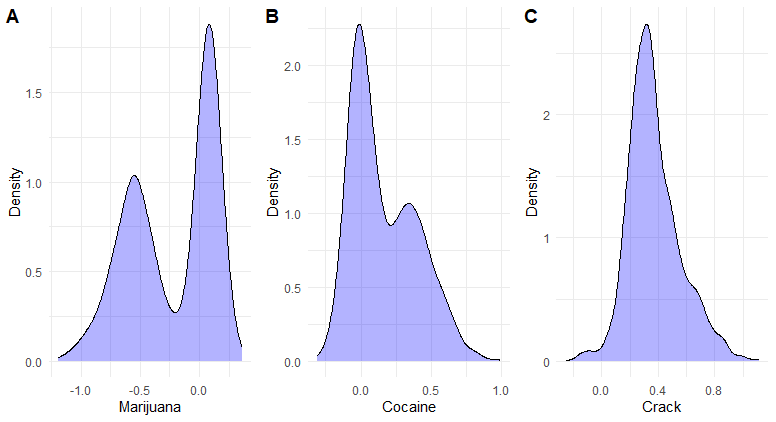
\includegraphics[width=340pt, height=200pt]{Chapters/chapter11/figures/ElastDrugs.png}
	\caption[List of figure caption goes here]{Posterior distributions: Elasticities of marijuana consumption in Colombia.}\label{figElastDrugs}
\end{figure}



\section{Splines}\label{sec11_2}

To clarify ideas, let's begin with a simple univariate case. The starting point is to assume that  
\[
y_i = f(x_{i}) + \mu_i,
\]  
where \(\mu_i \sim N(0, \sigma^2)\) is independent of the regressor \(x_{i}\), and \(f(x_{i})\) is a smooth function such that nearby points in the support of \(x_{i}\) should have similar values. The index \(i = 1,2,\dots, N\) represents the observations.  

The spline approach defines  
\begin{align}\label{eq11_1}
	f(x_{i}) = \beta_{1}b_1(x_{i}) + \beta_{2}b_2(x_{i}) + \dots + \beta_{H}b_H(x_{i}) = \boldsymbol{b}(x_{i})^{\top}\boldsymbol{\beta},
\end{align}  
where \(\boldsymbol{\beta} = [\beta_{1} \ \beta_{2} \ \dots \ \beta_{H}]^{\top}\) and \(\boldsymbol{b}(x_{i}) = [b_1(x_{i}) \ b_2(x_{i}) \ \dots \ b_H(x_{i})]^{\top}\) are the vector of parameters and the vector of spline basis (B-splines) function values at \(x_{i}\), respectively.  

Note that in this setting, there is only one regressor; however, there are \(H\) location parameters. Given \(N\) observations, the design matrix is:
\begin{align*}
	\boldsymbol{W}=\begin{bmatrix}
		b_1(x_{1}) & b_2(x_{1}) & \dots & b_H(x_{1})\\
		b_1(x_{2}) & b_2(x_{2}) & \dots & b_H(x_{2})\\
		\vdots & \vdots & \ddots & \vdots \\
		b_1(x_{N}) & b_2(x_{N}) & \dots & b_H(x_{N})\\
	\end{bmatrix}.
\end{align*} 
Thus, we have a standard linear model where we can proceed as in Chapter \ref{chap4}.

Actually, Equation \ref{eq11_1} represents the basis function approach, where \(\boldsymbol{b}(x_{i})\) is a specified set of basis functions, such as B-splines. However, other functions derived from the Fourier transform, Gaussian radial basis functions, wavelets, etc., can also be used. Here, we focus on the most popular case: cubic B-splines. However, the same ideas apply to other basis functions. In particular, cubic B-splines provide the lowest degree necessary to generate sufficiently smooth curves; the first and second derivatives are nonzero, which is not the case with constant and linear splines \cite{BMCP2021}.  

Thus, from Equation \ref{eq11_1}, we see that a spline is a linear combination of \(H\) B-splines. The latter are polynomials of a certain degree, meaning that splines are piecewise polynomial functions. Any spline function of order \(n\) can be expressed as a linear combination of B-splines of order \(n\), and B-splines serve as the basis functions for the spline function space.
%(https://en.wikipedia.org/wiki/B-spline#Cubic\_B-Splines)
The cubic B-spline is 
\begin{align*}
	b_{h,3}(x_i)=\begin{Bmatrix}
		\frac{u^3}{6} & x_h \leq x_i < x_{h+1}, & u=(x_i-x_h)/\delta\\
		\frac{1+3u+3u^2-3u^3}{6} & x_{h+1} \leq x_i < x_{h+2}, & u=(x_i-x_{h+1})/\delta\\
		\frac{4-6u^2+3u^3}{6} & x_{h+2} \leq x_i < x_{h+3}, & u=(x_i-x_{h+2})/\delta\\
		\frac{1-3u+3u^2-3u^3}{6} & x_{h+3} \leq x_i < x_{h+4}, & u=(x_i-x_{h+3})/\delta\\
		0 & \text{otherwise}
	\end{Bmatrix},
\end{align*}
where \(x_{h+k}\) are called the knots, for \(k=0,1,\dots,4\). These are the points in the domain of the function where the pieces of the spline join, satisfying \(x_{h+k} \leq x_{h+k+1}\). The knots control the shape and flexibility of the spline curve; more knots imply greater flexibility but less smoothness. Note that \(\delta\) determines the distance between the knots. This expression clearly shows that the cubic B-spline is a piecewise polynomial function.

The following code implements this function in \textbf{R} using a delta of 1.5 and 5 knots \( \left\{2, 3.5, 5, 6.5, 8\right\} \). The knots \( \left\{2, 8\right\} \) are called external knots, and the knots \( \left\{3.5, 5, 6.5\right\} \) are called internal knots. B-splines with evenly distributed knots are called uniform B-splines. However, this is not always the case.

Figure \ref{figCubicBspline} compares the results of our own function (black circles) with those obtained using the \textit{bs} function from the \textit{splines} package (red line).

\begin{tcolorbox}[enhanced,width=4.67in,center upper,
	fontupper=\large\bfseries,drop shadow southwest,sharp corners]
	\textit{R code. B-spline}
	\begin{VF}
		\begin{lstlisting}[language=R]
SplineOwn <- function(x, knots, delta){
	if(knots[1] <= x & x < knots[2]){
		u <- (x - knots[1])/delta
		b <- u^3/6
	}else{
		if(knots[2] <= x & x < knots[3]){
			u <- (x - knots[2])/delta
			b <- (1/6)*(1 + 3*u + 3*u^2 - 3*u^3)
		}else{
			if(knots[3] <= x & x < knots[4]){
				u <- (x - knots[3])/delta
				b <- (1/6)*(4 - 6*u^2 + 3*u^3)
			}else{
				if(knots[4] <= x & x < knots[5]){
					u <- (x - knots[4])/delta
					b <- (1/6)*(1 - 3*u + 3*u^2 - u^3)
				}else{
					b <- 0
				}
			}
		}
	}
	return(b)
}
delta <- 1.5
knotsA <- seq(2, 8, delta)
xA <- seq(2, 8, 0.1)
Ens <- sapply(xA, function(xi) {SplineOwn(xi, knots = knotsA, delta = delta)})
plot(xA, Ens, xlab = "x", ylab = "B-spline", main = "Cubic B-spline comparison: own function vs bs")
require(splines)
BSfunc <- bs(xA, knots = knotsA, degree = 3)
lines(xA, BSfunc[,4], col = "red")
\end{lstlisting}
	\end{VF}
\end{tcolorbox}

\begin{figure}[!h]
	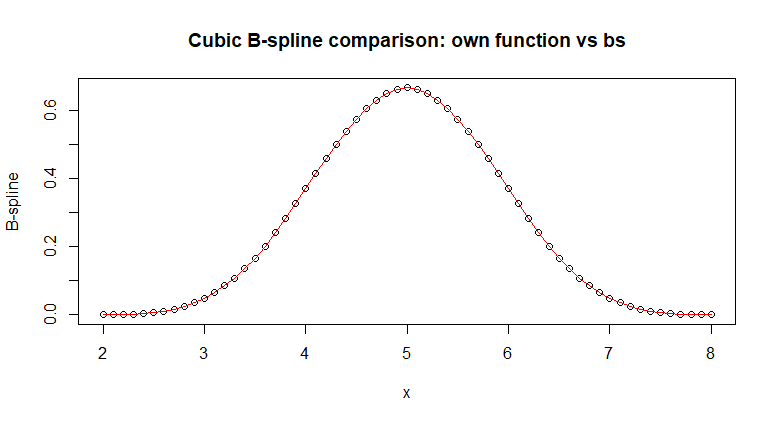
\includegraphics[width=340pt, height=200pt]{Chapters/chapter11/figures/CubicBspline.png}
	\caption[List of figure caption goes here]{Cubic B-spline comparison.}\label{figCubicBspline}
\end{figure}

Figure \ref{figCubicBspline} shows a particular cubic B-spline, but \( f(x_i) \) in Equation \ref{eq11_1} involves \( H \) splines over the range of potential values of \( x \), as we need to evaluate the splines centered at different knots. Here, we should clarify that to avoid issues with the use of splines at boundary regions, it is essential to artificially increase the number of external knots by repeating the external knots as many times as the degree of the polynomial. For instance, in our example, the final set of knots is \( \left\{2, 2, 2, 2, 3.5, 5, 6.5, 8, 8, 8, 8\right\} \). %However, the number of B-splines is based on the original set of knots. 
%. The number of B-splines is given by the number of knots plus the polynomial degree minus one (see Equation \ref{eq11_2} below)
%\footnote{In B-splines, the intercept (constant term) is generally not uniquely identified. Therefore, the common practice is to calculate the B-splines without the intercept and add the intercept in the regression (Equation \ref{eq11_1}). This implies using minus 2, rather than minus 1.}

The set of B-splines can be constructed using the Cox–de Boor recursion formula. The starting point is the B-spline of degree 0,
\begin{align*}
		b_{h,0}(x_i)=\begin{Bmatrix}
		1 & x_h \leq x_i < x_{h+1}, & u=(x_i-x_h)/\delta\\
		0 & \text{otherwise}
	\end{Bmatrix},
\end{align*}
and then, the other B-splines are defined by the recursion
\begin{align}\label{eq11_2}
	b_{h,p}(x_i)=\frac{x_i-x_{h}}{x_{h+p}-x_h}b_{h,p-1}(x_i)+\frac{x_{h+p+1}-x_i}{x_{h+p+1}-x_{h+1}}b_{h+1,p-1}(x_i).
\end{align}
The following code demonstrates how to perform this recursion using the same settings as in the previous code and compares the results with the \textit{bs} function from the \textit{splines} package. As shown in Figure \ref{figBsplines}, we obtain the same results. We will continue using the \textit{bs} function from the \textit{splines} package for convenience in the process, but it seems that we have gained some understanding of the underlying process.

\begin{tcolorbox}[enhanced,width=4.67in,center upper,
	fontupper=\large\bfseries,drop shadow southwest,sharp corners]
	\textit{R code. Splines}
	\begin{VF}
		\begin{lstlisting}[language=R]
cubic_bspline <- function(x, knots, degree = 3) {
	extended_knots <- c(rep(knots[1], degree), knots, rep(knots[length(knots)], degree))
	num_basis <- length(knots) + degree - 1  
	basis_matrix <- matrix(0, nrow = length(x), ncol = num_basis)
	# Function to compute B-spline basis recursively
	b_spline_basis <- function(x, degree, i, knots) {
		if (degree == 0) {
			return(ifelse(x >= knots[i] & x < knots[i + 1], 1, 0))
		} else {
			left_num <- (x - knots[i])
			left_den <- (knots[i + degree] - knots[i])
			left <- ifelse(left_den != 0, (left_num / left_den) * b_spline_basis(x, degree - 1, i, knots), 0)
			
			right_num <- (knots[i + degree + 1] - x)
			right_den <- (knots[i + degree + 1] - knots[i + 1])
			right <- ifelse(right_den != 0, (right_num / right_den) * b_spline_basis(x, degree - 1, i + 1, knots), 0)
			
			return(left + right)
		}
	}
	
	for (i in 1:num_basis) {
		basis_matrix[, i] <- sapply(x, function(xi) b_spline_basis(xi, degree, i, extended_knots))
	}
	if(x[length(x)] == knots[length(knots)]){
		basis_matrix[length(x), num_basis] <- 1
	}
	return(basis_matrix)
}
delta <- 1.5
knotsA <- seq(2, 8, delta)
xA <- seq(2, 8, 0.1)
basis_matrix <- cubic_bspline(xA, knots = knotsA, degree = 3)
library(splines)
bs_matrix <- bs(xA, knots = knotsA[-c(1, length(knotsA))], degree = 3, intercept = TRUE, Boundary.knots = range(knotsA))
bs_matrix_matrix <- as.matrix(bs_matrix)
par(mfrow = c(1,2))
matplot(xA, basis_matrix, type = "l", lty = 1, col = rainbow(ncol(basis_matrix)), ylab = "B-spline Basis", xlab = "x", main = "Own function")
matplot(xA, bs_matrix_matrix, type = "l", lty = 1, col = rainbow(ncol(basis_matrix)), ylab = "B-spline Basis", xlab = "x", main = "bs function")
\end{lstlisting}
	\end{VF}
\end{tcolorbox}

\begin{figure}[!h]
	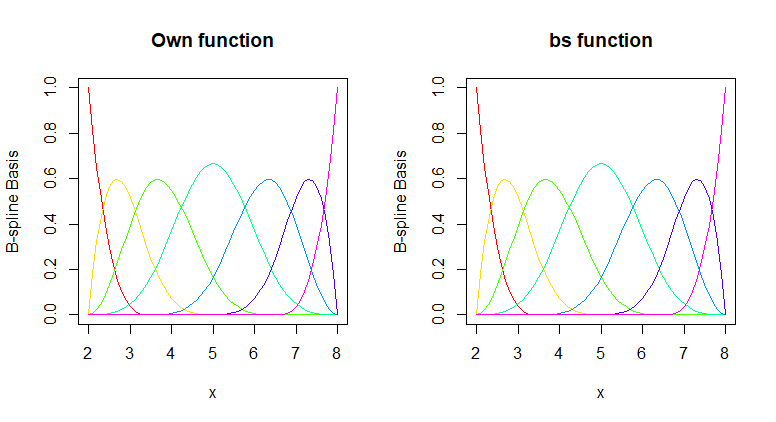
\includegraphics[width=340pt, height=200pt]{Chapters/chapter11/figures/Bsplines.png}
	\caption[List of figure caption goes here]{Sequence of cubic B-splines comparison.}\label{figBsplines}
\end{figure}

The idea in splines is to calculate the linear combination of the $H$ B-splines, as those shown in Figure \ref{figBsplines}, that bets fit the dependent variable. Let's perform a simulation exercise to fix ideas.\\

\textbf{Simulation exercise: Splines}

Let's assume that the data generating process is
\begin{align*}
	y_i & = 0.4 + 0.25\sin(8x_i - 5) + 0.4\exp(-16(4x_i - 2.5)^2) + \mu_i,
\end{align*}
where $\mu_i \sim N(0,0.15^2)$, and $x_i$ is a sequence in $(0,1)$, with 100 random draws of the pairs $(x_i, y_i)$. In addition, we choose the knots $\left\{0, 0.25, 0.5, 0.75, 1\right\}$. We then calculate the cubic B-splines, where the last column is 0, and the last two columns generate multicollinearity issues. Therefore, we exclude them when generating random realizations of splines by drawing the coefficients from $N(0, 0.35^2)$. The intercept is fixed to maintain the scale in Figure \ref{figRealizationBsplines}, where we can observe the data points, $f(x)$, and the different splines associated with various random realizations of the coefficients. The following code demonstrates how to perform this simulation.

\begin{tcolorbox}[enhanced,width=4.67in,center upper,
	fontupper=\large\bfseries,drop shadow southwest,sharp corners]
	\textit{R code. Realizations of splines}
	\begin{VF}
		\begin{lstlisting}[language=R]
########### Simulation: B-splines ###########
rm(list = ls())
library(ggplot2); library(splines)
set.seed(010101)
x <- seq(0, 1, 0.001)
ysignal <- 0.4 + 0.25*sin(8*x - 5) + 0.4*exp(-16*(4*x - 2.5)^2)
sig <- 0.15
e <- rnorm(length(ysignal), 0, sd = sig)
y <- ysignal + e
N <- 100
ids <- sort(sample(1:length(ysignal), N))
xobs <- x[ids]
yobs <- y[ids]
knots <- seq(0, 1, 0.25)
BS <- bs(xobs, knots = knots, degree = 3, Boundary.knots = range(x), intercept = FALSE)
# Splines
Spline1 <- 0.56 + BS[,-c(7:8)] %*% rnorm(6, 0, 0.35)
Spline2 <- 0.56 + BS[,-c(7:8)] %*% rnorm(6, 0, 0.35)
Spline3 <- 0.56 + BS[,-c(7:8)] %*% rnorm(6, 0, 0.35)
Spline4 <- 0.56 + BS[,-c(7:8)] %*% rnorm(6, 0, 0.35)
# Create data frames for the true signal, observed data, and Splines
data_true_signal <- data.frame(x = x, y = ysignal, Type = "True Signal")
data_obs <- data.frame(x = xobs, y = yobs, Type = "Observed Data")
# Create separate data frames for each Spline
data_Spline1 <- data.frame(x = xobs, y = Spline1, Type = "Spline 1")
data_Spline2 <- data.frame(x = xobs, y = Spline2, Type = "Spline 2")
data_Spline3 <- data.frame(x = xobs, y = Spline3, Type = "Spline 3")
data_Spline4 <- data.frame(x = xobs, y = Spline4, Type = "Spline 4")
data <- rbind(data_true_signal, data_obs, data_Spline1, data_Spline2, data_Spline3, data_Spline4)
ggplot(data, aes(x = x, y = y)) + geom_line(data = subset(data, Type == "True Signal"), aes(color = "True Signal"), linewidth = 1) + geom_point(data = subset(data, Type == "Observed Data"), aes(color = "Observed Data"), shape = 16) + geom_line(data = subset(data, Type == "Spline 1"), aes(color = "Splines"), linewidth = 1, linetype = "solid") + geom_line(data = subset(data, Type == "Spline 2"), aes(color = "Splines"), linewidth = 1, linetype = "solid") + geom_line(data = subset(data, Type == "Spline 3"), aes(color = "Splines"), linewidth = 1, linetype = "solid") + geom_line(data = subset(data, Type == "Spline 4"), aes(color = "Splines"), linewidth = 1, linetype = "solid") + scale_color_manual(values = c("True Signal" = "black", "Observed Data" = "red", "Splines" = "blue")) + labs(y = "y", color = "Legend") + theme_minimal() +
theme(legend.position = "top")
\end{lstlisting}
	\end{VF}
\end{tcolorbox}

\begin{figure}[!h]
	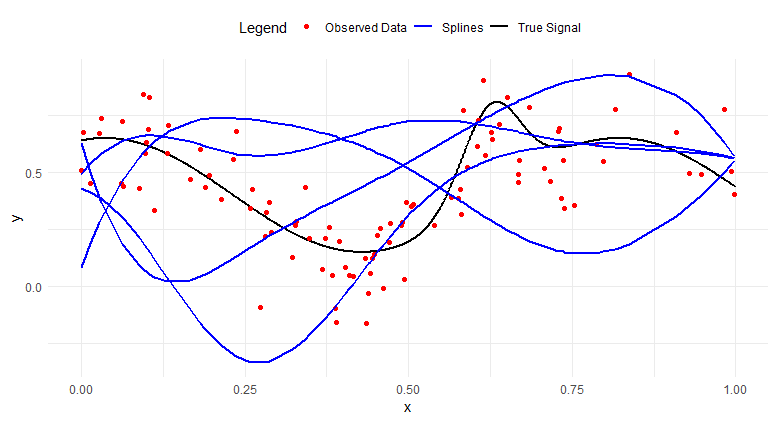
\includegraphics[width=340pt, height=200pt]{Chapters/chapter11/figures/RealizationsSplines.png}
	\caption[List of figure caption goes here]{Different realizations of splines.}\label{figRealizationBsplines}
\end{figure}

We can also use this simulation to examine the effect of changing the knots. The following code performs the fit using least squares, which is equivalent to using a non-informative prior in a Bayesian linear regression framework.

Figure \ref{figFitBsplines} illustrates the fit of different splines based on varying numbers of knots. We observe that increasing the number of knots enhances the flexibility of the spline, providing better local control. However, too many knots can result in a wiggly, overly complex fit that captures noise rather than the true underlying trend and may also increase multicollinearity. Therefore, selecting an appropriate number of knots is a crucial aspect of spline modeling. To address this issue, we can apply the strategies discussed in Chapter \ref{chap10}, and the strategies that will be discussed in Section \ref{sec13_2} in the next chapter. 

\begin{tcolorbox}[enhanced,width=4.67in,center upper,
	fontupper=\large\bfseries,drop shadow southwest,sharp corners]
	\textit{R code. Fit using splines: Different knots}
	\begin{VF}
		\begin{lstlisting}[language=R]
rm(list = ls())
library(ggplot2); library(splines)
# Data generation
set.seed(10101)
x <- seq(0, 1, 0.001)
ysignal <- 0.4 + 0.25*sin(8*x - 5) + 0.4*exp(-16*(4*x - 2.5)^2)
sig <- 0.15; e <- rnorm(length(ysignal), 0, sd = sig)
y <- ysignal + e; N <- 100
ids <- sort(sample(1:length(ysignal), N))
xobs <- x[ids]
yobs <- y[ids]
# Generate Fits with different knot placements
knots_list <- list(seq(0, 1, 0.33), seq(0, 1, 0.25), seq(0, 1, 0.2), seq(0, 1, 0.1))
Fits <- list()
for (i in 1:4) {
	BS <- bs(xobs, knots = knots_list[[i]], degree = 3, Boundary.knots = range(x), intercept = FALSE)
	fm <- lm(yobs ~ BS)
	Fits[[i]] <- predict(fm)
}
# Create data frames
data_true_signal <- data.frame(x = x, y = ysignal, Type = "True Signal")
data_obs <- data.frame(x = xobs, y = yobs, Type = "Observed Data")
data_preds <- data.frame(
x = rep(xobs, 4),
y = c(Fits[[1]], Fits[[2]], Fits[[3]], Fits[[4]]),
Type = rep(c("Fit 1", "Fit 2", "Fit 3", "Fit 4"), each = length(xobs))
)
data <- rbind(data_true_signal, data_obs, data_preds)

# Create ggplot
ggplot(data, aes(x = x, y = y, color = Type)) + geom_line(data = subset(data, Type == "True Signal"), linewidth = 1) + geom_point(data = subset(data, Type == "Observed Data"), shape = 16, size = 2) + geom_line(data = subset(data, grepl("Fit", Type)), linewidth = 1, linetype = "solid") + scale_color_manual(values = c("True Signal" = "black", "Observed Data" = "red", "Fit 1" = "blue", "Fit 2" = "green", "Fit 3" = "orange", "Fit 4" = "purple")) + labs(y = "y", color = "Legend") +
theme_minimal() + theme(legend.position = "top")
\end{lstlisting}
	\end{VF}
\end{tcolorbox}

\begin{figure}[!h]
	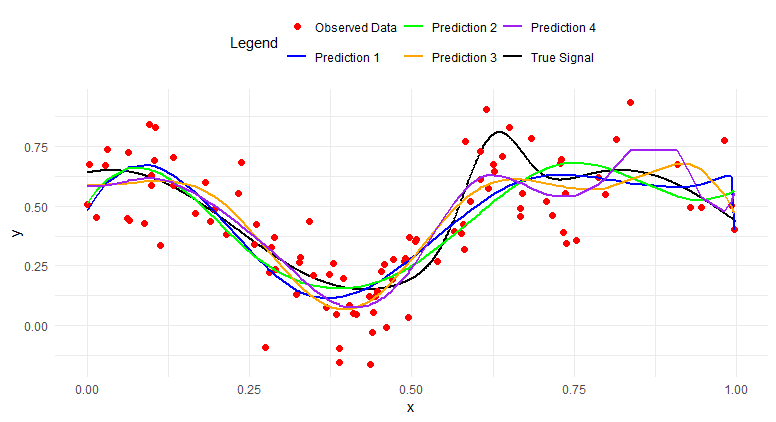
\includegraphics[width=340pt, height=200pt]{Chapters/chapter11/figures/SplineFit.png}
	\caption[List of figure caption goes here]{Different fits of splines.}\label{figFitBsplines}
\end{figure}

Note that splines use local information to perform the fit. This implies the \textit{curse of dimensionality} issue, where increasing the number of variables leads to more dispersed regions in the regressor space. In other words, the observations become increasingly further apart as we have more regressors. As a result, splines become less reliable in high-dimensional spaces.

A strategy to overcome the curse of dimensionality is to specify the \textit{partial linear model}: 
\begin{align*} 
	y_i & = \boldsymbol{z}_i^{\top}\boldsymbol{\gamma} + f(x_i) + \mu_i. 
\end{align*} 
In this specification, some regressors enter in a linear way, while the most relevant regressor — the one under primary investigation — enters in a non-parametric way. Note that we only need to increase the dimension of the matrix $\boldsymbol{W}$ by adding the columns from $\boldsymbol{z}$, and proceed as we did previously.

\begin{itemize}
	\item Show cubic B-spline (own function using Equation 20.2 in \cite{gelman2021bayesian})
	\item Show sequence of cubic B-splines (function from chatGPB and bs function)
	\item Then using bs function from R. Simulate splines with draws from normal distribution (first do next to know reasonable values)
	\item Simulate function in $f(x_i)=0.4+0.25 \sin(8x_i-5)+0.4\exp\left\{-16(4x_i-2.5)^2\right\}$ \cite{Otsu2017} or page 251 \cite{koop2003bayesian}, and check performance with different knots, figure 5.10 in \cite{BMCP2021}
	\item Selection of $H$, or check section 20.2 in \cite{gelman2021bayesian}, and 5.5 and 5.6 in \cite{BMCP2021}. Selection of $H$ is a problem of variable selection (regressors uncertainty), and can be handle using the approach in Chapter 10. Other approaches, like the ones in the regularization section in the following chapter can be used (Bayesian LASSO, SSVS, etc.) 
	\item Partial linear model due to curse of dimensionality. Check \cite{koop2003bayesian}
	\item Application marijuana, own price elasticity	
\end{itemize}



%\subsection{Partial linear model}\label{sec11_21}

\section{Summary}\label{sec11_3}

\section{Exercises}\label{sec11_4}

\begin{enumerate}
	\item Simulate a semi-parametric regression where  
	\begin{align*}
		y_i &= 0.5x_{i1} - 1.2x_{i2} + \mu_i, \\
		p(\mu_i) &= 
		0.3 \phi(\mu_i \mid -0.5,0.5^2) + 0.7 \phi(\mu_i \mid 1,0.8^2).		
	\end{align*}
	Assume that $x_{i1}$ and $x_{i2}$ follow a standard normal distribution and that the sample size is 1,000. Perform inference in this model assuming that the number of components is unknown. Start with $H=5$ and use non-informative priors, setting $\alpha_{h0}=\delta_{h0}=0.01$, $\boldsymbol{\beta}_0=\boldsymbol{0}_2$, $\boldsymbol{B}_0=\boldsymbol{I}_2$, $\mu_{h0}=0$, $\sigma^2_{\mu 0}=10$, and $\boldsymbol{\alpha}_0=[1/H \ \dots \ 1/H]^{\top}$. Use 6,000 MCMC iterations, a burn-in period of 4,000, and a thinning parameter of 2. Compare the population parameters with the posterior estimates and plot the population density along with the posterior density estimate of $\boldsymbol{\mu}$ (the mean, and the 95\% credible interval).
	
	\item \textbf{Example: Consumption of marijuana in Colombia continues I}
	
	Use the dataset \textit{MarijuanaColombia.csv} from our GitHub repository to perform inference on the demand for marijuana in Colombia. This dataset contains information on the (log) monthly demand in 2019 from the National Survey of the Consumption of Psychoactive Substances. It includes variables such as the presence of a drug dealer in the neighborhood (\textit{Dealer}), gender (\textit{Female}), indicators of good physical and mental health (\textit{PhysicalHealthGood} and \textit{MentalHealthGood}), age (\textit{Age} and \textit{Age2}), and (log) prices of marijuana, cocaine, and crack by individual (\textit{LogPriceMarijuana}, \textit{LogPriceCocaine}, and \textit{LogPriceCrack}). The sample size is 1,156.
	
	Estimate a finite Gaussian mixture regression using non-informative priors, that is, $\alpha_{0}=\delta_{0}=0.01$, $\boldsymbol{\beta}_{0}=\boldsymbol{0}_K$, $\boldsymbol{B}_{0}=\boldsymbol{I}_K$, and $a=b=0.1$, $K$ is the number of regressors, 10 including the intercept. The number of MCMC iterations is 5,000, the burn-in is 1,000, and the thinning parameter is 2. Start with five potential clusters. Obtain the posterior distribution of the own-price elasticity of marijuana and the cross-price elasticities of marijuana demand with respect to the prices of cocaine and crack.
	
	\item Get the posterior sampler in the semi-parametric setting using a Dirichlet process mixture:
	\begin{align*}
		y_i&=\boldsymbol{x}_i^{\top}\boldsymbol{\beta}+e_i\\
		e_i\mid \mu_i,\sigma_i^2 &\stackrel{iid}{\sim} N(\mu_i,\sigma_i^2),
	\end{align*}
	Do not include the intercept in $\boldsymbol{\beta}$ to get flexibility in the distribution of the stochastic errors.
	
	Let's assume $\boldsymbol{\beta}\sim N(\boldsymbol{\beta}_0,\boldsymbol{B}_0)$, $\sigma_i^2\sim IG(\alpha_0/2,\delta_0/2)$, $\mu_i\sim N(\mu_0,\sigma_i^2/\beta_0)$, $\alpha\sim G(a,b)$ such that introducing the latent variable $\xi|\alpha,N\sim Be(\alpha+1,N)$, allows to easily sample the posterior draws of  $\alpha|\xi,H,\pi_{\xi}\sim\pi_{\xi}{G}(a+H,b-log(\xi))+(1-\pi_{\xi}){G}(a+H-1,b-log(\xi))$, where $\frac{\pi_{\xi}}{1-\pi_{\xi}}=\frac{a+H-1}{N(b-log(\xi))}$, $H$ is the number of atoms (mixture components). 
	
	\item  \textbf{Example: Exercise 1 and 3 continue}
	
	Perform inference in the simulation of the semi-parametric model of Exercise 1 using the sampler of Exercise 3. Use non-informative priors, setting $\alpha_{0}=\delta_{0}=0.01$, $\boldsymbol{\beta}_{0}=\boldsymbol{0}_2$, $\boldsymbol{B}_{0}=\boldsymbol{I}_2$, and $a=b=0.1$. The number of MCMC iterations is 5,000, the burn-in is 1,000, and the thinning parameter is 2. 
	
	\item \textbf{Example: Simulation exercise continues}
	
	Fix the label-switching problem of the simulation exercise of the DPM using \textit{random permutation of latent classes}.
	
	\item \textbf{Example: Consumption of marijuana in Colombia continues II}
	
	Perform the application of marijuana consumption with the following specification:
	\begin{align*}
		y_i & = \boldsymbol{z}_i^{\top} \boldsymbol{\gamma} + f(\log(p)_{im}) + f(\log(p)_{ic}) + f(\log(p)_{ib}) + \mu_i,
	\end{align*}
	where $\boldsymbol{z}_i$ represents the presence of a drug dealer in the neighborhood (\textit{Dealer}), gender (\textit{Female}), indicators of good physical and mental health (\textit{PhysicalHealthGood} and \textit{MentalHealthGood}), and age (\textit{Age} and \textit{Age2}), and $\log(p)_{im}$, $\log(p)_{ic}$, and $\log(p)_{ib}$ are the (log) prices of marijuana, cocaine, and crack by individual.
	
	Implement a strategy that retains the drug prices in the regression, selects the number of knots using the BIC approximation, and also uses the BIC approximation to select the other regressors.
	
  
\end{enumerate}

